\documentclass[12pt, a4paper, oneside]{ctexart}
\usepackage{amsmath, amsthm, amssymb, bm, color, graphicx, geometry, mathrsfs,extarrows, braket, booktabs, array, xcolor, fontspec, appendix, float, wrapfig, enumitem, titlesec, titling, fancyhdr, algorithm, makecell, multirow}
\usepackage[colorlinks,linkcolor=red,anchorcolor=blue,citecolor=blue,urlcolor=blue,menucolor=black]{hyperref}
\usepackage{caption}
\usepackage{subcaption}
\usepackage{tocloft}

%%%% 设置中文字体 %%%%
% fc-list -f "%{family}\n" :lang=zh >d:zhfont.txt 命令查看已有字体
\setCJKmainfont[
    % BoldFont=方正新书宋_GBK,  % 粗体
    BoldFont=方正宋黑简体,  % 粗体
    ItalicFont=方正楷体_GBK,  % 楷体
    BoldItalicFont=方正粗楷简体,  % 粗楷体
    Mapping = fullwidth-stop  % 将中文句号“.”全部转化为英文句号“.”,
]{方正书宋简体}  % !!! 注意在Windows中运行请改为“方正书宋简体.ttf” !!!
%%%% 设置英文字体 %%%%
\setmainfont{Times New Roman}
\setsansfont{Calibri}
\setmonofont{Consolas}

%%%% 设置代码块 %%%%
% 在vscode中使用minted需要先配置python解释器, Ctrl+Shift+P, 输入Python: Select Interpreter选择安装了Pygments的Python版本. 再在setting.json中xelatex和pdflatex的参数中加入 "--shell-escape", 即可
% TeXworks中配置方法参考: https://blog.csdn.net/RobertChenGuangzhi/article/details/108140093
\usepackage{minted}
\renewcommand{\theFancyVerbLine}{
    \sffamily\textcolor[rgb]{0.5,0.5,0.5}{\scriptsize\arabic{FancyVerbLine}}} % 修改代码前序号大小
% 加入不同语言的代码块
\newmintinline{cpp}{fontsize=\small, linenos, breaklines, frame=lines}
\newminted{cpp}{fontsize=\small, baselinestretch=1, linenos, breaklines, frame=lines}
\newmintedfile{cpp}{fontsize=\small, baselinestretch=1, linenos, breaklines, frame=lines}
\newmintinline{matlab}{fontsize=\small, linenos, breaklines, frame=lines}
\newminted{matlab}{fontsize=\small, baselinestretch=1, mathescape, linenos, breaklines, frame=lines}
\newmintedfile{matlab}{fontsize=\small, baselinestretch=1, linenos, breaklines, frame=lines}
\newmintinline{python}{fontsize=\small, linenos, breaklines, frame=lines, python3}  % 使用\pythoninline{代码}
\newminted{python}{fontsize=\small, baselinestretch=1, linenos, breaklines, frame=lines, python3}  % 使用\begin{pythoncode}代码\end{pythoncode}
\newmintedfile{python}{fontsize=\small, baselinestretch=1, linenos, breaklines, frame=lines, python3}  % 使用\pythonfile{代码地址}

%%%% 设置行间距与页边距 %%%%
\linespread{1.2}
\geometry{left=2.5cm, right=2.5cm, top=2.5cm, bottom=2.5cm}
% \geometry{left=1.84cm,right=1.84cm,top=2.18cm,bottom=2.18cm}  % 更小的页边距

%%%% 设置页眉 %%%%
\pagestyle{fancy}
%\fancyhead[C]{\small\it\leftmark}
\fancyhead[L]{\small\it\leftmark}
\fancyhead[R]{\small\it 西安交通大学大学生创新训练项目结题报告}

%%%% 定理类环境的定义 %%%%
\newtheorem{example}{例}            % 整体编号
\newtheorem{theorem}{定理}[section] % 定理按section编号
\newtheorem{definition}{定义}
\newtheorem{axiom}{公理}
\newtheorem{property}{性质}
\newtheorem{proposition}{命题}
\newtheorem{lemma}{引理}
\newtheorem{corollary}{推论}
\newtheorem{condition}{条件}
\newtheorem{conclusion}{结论}
\newtheorem{assumption}{假设}
\numberwithin{equation}{section}  % 公式按section编号 (公式右端的小括号)

%%%% 自定义环境 %%%%
\newsavebox{\nameinfo}
\newenvironment{myTitle}[1]{
    \begin{center}
    {\zihao{-2}\bf #1\\}
    \zihao{-4}\it
}{\end{center}}  % \begin{myTitle}{标题内容}作者信息\end{myTitle}
\newcounter{problem}  % 问题序号计数器
\newenvironment{problem}[1][]{\stepcounter{problem}\par\noindent\textbf{题目\arabic{problem}. #1}}{\smallskip\par}
\newenvironment{solution}[1][]{\par\noindent\textbf{#1解答. }}{\smallskip\par}  % 可带一个参数表示题号\begin{solution}{题号}
\newenvironment{note}{\par\noindent\textbf{注记. }}{\smallskip\par}
\newenvironment{remark}{\begin{enumerate}[label=\textbf{注\arabic*.}]}{\end{enumerate}}
\BeforeBeginEnvironment{minted}{\vspace{-0.5cm}}  % 缩小minted环境距上文间距
\AfterEndEnvironment{minted}{\vspace{-0.2cm}}  % 缩小minted环境距下文间距

%%%% 自定义段落开头序号,间距 (titlesec) %%%%
% 中文序号:\zhnum{section}, 阿拉伯序号:\arabic
% \titleformat{\section}{\Large\bfseries}{\arabic{section}}{1em}{}[]
\titlespacing{\section}{0pt}{1.2ex plus .0ex minus .0ex}{.6ex plus .0ex}
\titlespacing{\subsection}{0pt}{1.2ex plus .0ex minus .0ex}{.6ex plus .0ex}
\titlespacing{\subsubsection}{0pt}{1.2ex plus .0ex minus .0ex}{.6ex plus .0ex}

%%%% 图片相对路径 %%%%
\graphicspath{{figures/}} % 当前目录下的figures文件夹, {../figures/}则是父目录的figures文件夹
\setlength{\abovecaptionskip}{0.5ex}  % 缩紧图片标题与图片之间的距离
\setlength{\belowcaptionskip}{0pt} 

%%%% 缩小item,enumerate,description两行间间距 %%%%
\setenumerate[1]{itemsep=0pt,partopsep=0pt,parsep=\parskip,topsep=5pt}
\setitemize[1]{itemsep=0pt,partopsep=0pt,parsep=\parskip,topsep=5pt}
\setdescription{itemsep=0pt,partopsep=0pt,parsep=\parskip,topsep=5pt}

%%%% 目录后面加上点点 %%%%
\renewcommand{\cftsecleader}{\cftdotfill{\cftdotsep}}

%%%% 自定义公式 %%%%
\everymath{\displaystyle} % 默认全部行间公式, 想要变回行内公式使用\textstyle
\DeclareMathOperator*\uplim{\overline{lim}}     % 定义上极限 \uplim_{}
\DeclareMathOperator*\lowlim{\underline{lim}}   % 定义下极限 \lowlim_{}
\DeclareMathOperator*{\argmax}{arg\,max}  % 定义取最大值的参数 \argmax_{}
\DeclareMathOperator*{\argmin}{arg\,min}  % 定义取最小值的参数 \argmin_{}
\let\leq=\leqslant % 简写小于等于\leq (将全部leq变为leqslant)
\let\geq=\geqslant % 简写大于等于\geq (将全部geq变为geqslant)
\DeclareRobustCommand{\rchi}{{\mathpalette\irchi\relax}}
\newcommand{\irchi}[2]{\raisebox{\depth}{$#1\chi$}} % 使用\rchi将\chi居中

%%%% 一些宏定义 %%%%
\def\bd{\boldsymbol}        % 加粗(向量) boldsymbol
\def\disp{\displaystyle}    % 使用行间公式 displaystyle(默认)
\def\tsty{\textstyle}       % 使用行内公式 textstyle
\def\sign{\text{sign}}      % sign function
\def\wtd{\widetilde}        % 宽波浪线 widetilde
\def\R{\mathbb{R}}          % Real number
\def\N{\mathbb{N}}          % Natural number
\def\Z{\mathbb{Z}}          % Integer number
\def\Q{\mathbb{Q}}          % Rational number
\def\C{\mathbb{C}}          % Complex number
\def\K{\mathbb{K}}          % Number Field
\def\P{\mathbb{P}}          % Polynomial
\def\E{\mathbb{E}}          % Exception
\def\d{\mathrm{d}}          % differential operator
\def\e{\mathrm{e}}          % Euler's number
\def\i{\mathrm{i}}          % imaginary number
\def\re{\mathrm{Re}}        % Real part
\def\im{\mathrm{Im}}        % Imaginary part
\def\res{\mathrm{Res}}      % Residue
\def\ker{\mathrm{Ker}}      % Kernel
\def\vspan{\mathrm{vspan}}  % Span  \span与latex内核代码冲突改为\vspan
\def\L{\mathcal{L}}         % Loss function
\def\O{\mathcal{O}}         % big O notation
\def\wdh{\widehat}          % 宽帽子 widehat
\def\ol{\overline}          % 上横线 overline
\def\ul{\underline}         % 下横线 underline
\def\add{\vspace{1ex}}      % 增加行间距
\def\del{\vspace{-1.5ex}}   % 减少行间距

%%%% 正文开始 %%%%
\begin{document}

%%%% 定义标题页,包括title,author,affiliation,email等 %%%%
\title{
    \vspace{2cm}
    
\includegraphics[width=7cm]{XJTU_logo}\\[1ex]
    \textbf{大学生创新训练项目\\[1ex]
    结题报告书} \vspace{3cm}
}
\preauthor{\begin{flushleft}\large}
\postauthor{\end{flushleft}}
\author{
    \hspace{3cm}\begin{minipage}[t]{0.65\linewidth}
\makebox[5em][s]{\textbf{项目名称:}}基于多元数据分析的重症监护室\\
\makebox[5em][s]{}病人健康状态预警方法研究\\[1ex]
\makebox[5em][s]{\textbf{起止年月:}}2022年5月至2023年5月\\[1ex]
\makebox[5em][s]{\textbf{负责人:}}喻彭\\[1ex]
\makebox[5em][s]{\textbf{手机:}}13036784398\\[1ex]
\makebox[5em][s]{\textbf{邮箱:}}yupeng666@stu.xjtu.edu.cn\\[1ex]
\makebox[5em][s]{\textbf{项目成员:}}吴天阳,王承杰\\[1ex]
\makebox[5em][s]{\textbf{指导老师:}}孙剑\\[1ex]
\makebox[5em][s]{\textbf{批准经费:}}10000\ \ \textbf{已用金额:}631.12\\[1ex]
\makebox[5em][s]{\textbf{填报日期:}}\today
    \end{minipage}
}
\date{\vspace{-22cm}\hspace{-12cm}\textbf{项目编号:}S202210698280}
\maketitle % 设置上面的标题
\fancypagestyle{titlestyle}{\pagestyle{empty}}
\thispagestyle{titlestyle}
\clearpage % 创建新的一面
\fancypagestyle{abstructstyle}{\fancyhf{}\fancyhead[C]{\small\it 摘要}}
\thispagestyle{abstructstyle}
\noindent\textbf{报告题目:基于多元数据分析的重症监护室病人健康状态预警方法研究}\\
\textbf{学生姓名:喻彭,吴天阳,王承杰}\\
\textbf{指导老师:孙剑}\\[1em]

\textbf{中文摘要}:医疗实践活动产生海量的数据,随着信息化的发展,我们得以及时记录医疗数据,
然而医疗重症监护数据是一个没有显著规律的动态系统, 数据随时间波动复杂变化,而且存在数据稀疏性强、
不规则程度高等问题。因此数据以往没有得到充分利用于临床诊断。我们以脓毒症(可导致 SIC 、DIC)为例,
获取了重症监护室记录MIMIC-IV数据集,对其进行筛选、异常值排查、数据缺失处理、实时状态标定等预处理,
使用随机梯度下降优化的线性模型(SGD)、SVM 模型、决策树、随机森林、K 近邻等机器学习方法进行模型构建,
用K-折交叉验证准确率、测试集准确率 和AUC等指标分析相关结果。
对于 DIC,我们发现在序列长度为 2、时间段长度为 4h 时,模型准确率较高;
对于 SIC 综合考虑,我们发现在序列长度为 3、时间段长度为 8h 时,模型效果较好。
最后用 SHAP 方法进行解释性分析,分别得到整体数据集的可解释性分析,并发现由SHAP给出的重要度与随机森林模型给出的重要度排名几乎相同,
说明SHAP确实能够对模型进行有效的数据解释;进一步,我们从标签对应的数据集中各取出一个数据进行具体可解释性分析,
并根据结果对患者的治疗方向提出建议。

\textbf{英文摘要}:Medical practice generates massive data. With the development of information technology, 
we can record medical data in real-time. However, ICU data is a dynamic system without significant 
patterns and has problems such as sparsity and irregularity. Therefore, it has not been fully 
utilized for clinical diagnosis. We used the MIMIC-IV dataset to build models using machine learning 
methods and analyzed the results with accuracy and AUC. We found that the model accuracy was higher 
for DIC when the sequence length was 2 and the time period was 4h, and for SIC when the sequence 
length was 3 and the time period was 8h. Finally, we used SHAP for interpretability analysis.

\textbf{关键词}:医疗数据分析,机器学习方法,可解释性分析。
\clearpage
\fancypagestyle{tablestyle}{\fancyhf{}\fancyhead[C]{\small\it 目录}}
\thispagestyle{tablestyle}
\tableofcontents % 创建目录页,使用目录需要编译两次, 并且不能删去编译产生的临时文件!!!

%%%% 以下部分是正文 %%%%  
\clearpage
\setcounter{page}{1}
\section{绪论}
医疗实践活动产生海量的数据,随着信息化的发展,我们得以及时记录医疗数据,深度挖掘和利用这些数据对提高医疗、护理质量以及患者安全都具有重大意义。
本项目拟以脓毒症为例,收集重症监护室记录数据,对其进行筛选、异常值排查、数据缺失处理、标记等预处理,
设计多种涵盖机器学习方法进行模型构建,分析相关结果并进行验证。
搭建实时的检测预警系统,预测患者患病风险,为医生诊断提供有效参考。

近些年来,机器学习对脓毒症的早期预测有了极大的进展。2018年,Nemati 等根据纳入患者实时监测的 EMR 数据中提取的 65 个变量,
机器学习构建出了人工智能脓毒症专家(artificial intelligence sepsis expert,AISE)预警模型,
可以优先临床 4-12 h 预测脓毒症的发生。2020年,Burdick等根据270 438例住院或急诊成人患者的心率、呼吸频率、收缩压、舒张压、体温、血氧饱和度,
利用梯度增强方法所开发的预警模型就可以提前48 h预测脓毒症的发生。2020年,Yang等利用极端梯度增强(eXtreme Gradient Boosting,XGBoost)
算法提取了34 285 例成人重症患者 EHR 数据中的168个临床特征变量,并训练出了一个可解释的人工智 能脓毒症预测模型(explainable AI sepsispredictor,EASP),
该模型能够提前预测脓毒症患病风险。

通过机器学习继续提高脓毒症早期预测的时间和精确性是非常值得研究的问题,将会降低脓毒症的治疗成本改善结果,并为医疗系统、医务人员和患者带来极大的益处。

本文将基于MIMIC-IV 2.2数据集对299 712位病人的住院及化验信息,提取与脓毒症判断相关的信息,并对数据进行插补、异常值矫正、缺失值处理后,
使用不同的机器学习模型对病人是否患有DIC进行预测,使用K-折交叉验证并用ROC对模型进行评估,从而得到最优的模型与数据集处理方法,
最后使用SHAP值对模型的可解释性进行分析,以解释不同的特征对最终预测结果的影响。
\clearpage
\section{数据集分析及预处理}
\subsection{数据集介绍}
我们已在PhysioNet上获取了MIMIC数据集使用权限,使用的为当前最新的MIMIC-IV 2.2数据集\cite{bib-mimic,bib-mimic-origin},
该数据集在之前的基础上修复了部分错误,并加入了护理信息。

MIMIC-IV数据集通过医院中的数字电子健康记录系统(Electronic Health Recor system, EHR)对全部入院病人信息进行记录,
通过BIDMC的MetaVision(iMDSoft)系统对ICU病人的生命体征数据进行记录,出于对患者隐私的保护,全部患者姓名与入院年份均经过Hash编码,
通过对数据的大致分析,我们得到入院病人总数为$299712$人,住院病人$180733$人,ICU病人$50920$人。图\ref{fig-age}中分别显示了
入院与进入ICU的年龄占比分布,并通过分析得到该数据集中进入医院的病人中死亡率为$9.70\%$,而进入ICU病人的死亡率为$32.36\%$,基本符合实际情况。
\begin{figure}[H]
    \vspace{-1em}
    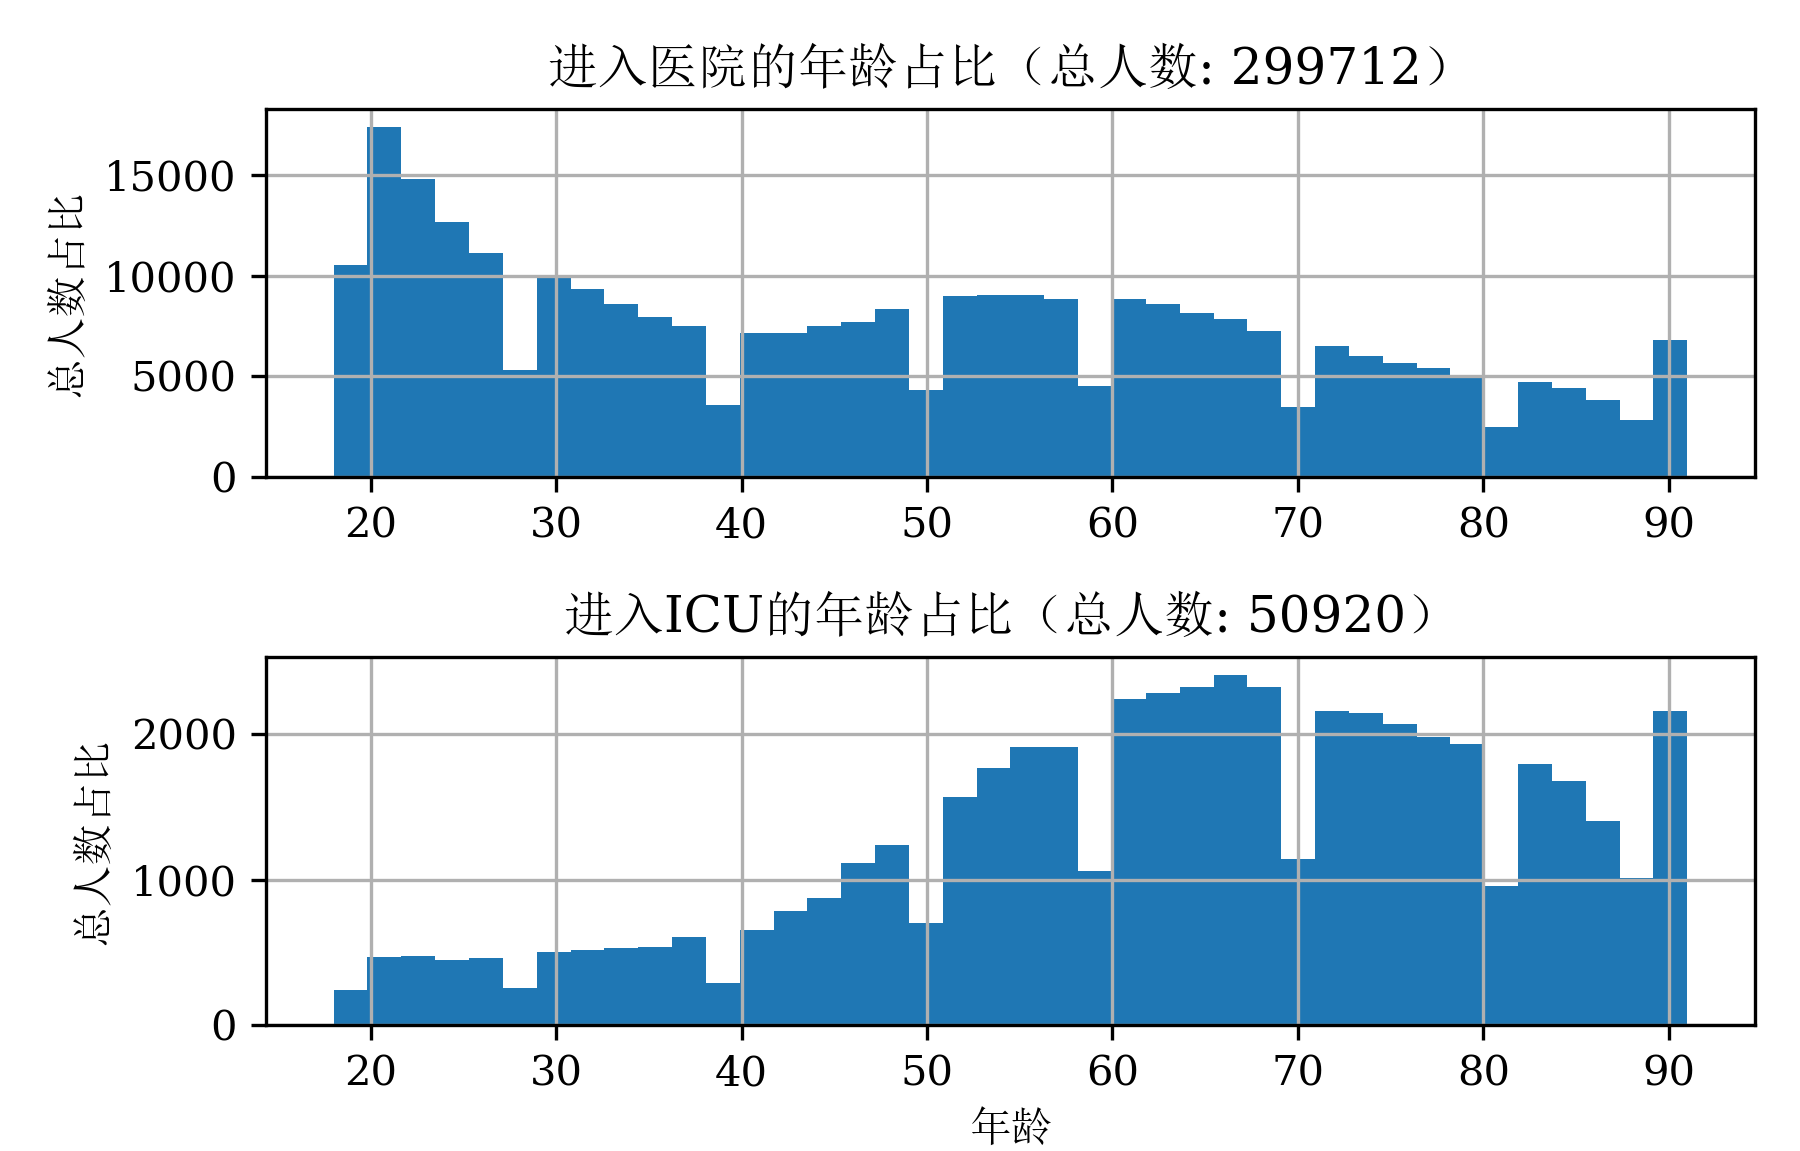
\includegraphics[width=\textwidth]{admission_vs_age_plot.png}
    \caption{数据集中年龄占比分布}
    \label{fig-age}
\end{figure}
\subsection{数据预处理}
\subsubsection{数据提取}
由于MIMIC-IV中的数据都是每次的化验结果,我们首先要找到与DIC症状相关的化验信息,并将所有相关化验信息整合在一起,
基于文献\cite{bib-determine-dic}中给出的信息,我们将表\ref{table-id}中的8个化验信息作为判断脓毒症的特征。
其中前5项与DIC的判定有关,后3项为常见化验项目,用于发现与DIC可能存在的潜在关系。

经过分析处理后,我们得到如图\ref{fig-capture},两个图分别显示了每种标签的化验条例数目和每个时刻下的检测数据中所包含的非空条例数目。
从图中不难看出,D-Dim的条例数目最少,很有可能是因为该化验只会对感染某些与呼吸道相关疾病时才会检验,从第二个图中可以看出
大多数的时刻下的数据都只包含3个特征数据,所以我们首先需要按照一个时间短对数据进行插补。

% \renewcommand\arraystretch{1} % 设置表格高度为原来的0.8倍
\begin{table}[H] % table标准
    \centering % 表格居中
    \begin{tabular}{p{0.4\textwidth}<{\raggedright}p{0.2\textwidth}<{\centering}p{0.3\textwidth}} % 设置表格宽度
        \toprule
        \textbf{数据全称}&\textbf{缩写}&\textbf{MIMIC-IV数据编号}\\
        \midrule
        1. 血小板计数(Platelet Count)&PLT&227457\\
        2. 凝血酶原时间(Prothrombin time)&PT&227465\\
        \makecell[l]{3.凝血酶原时间的国际标准化比值\\ \makebox[2ex][]{}(International Normalized Ratio)}&INR&227467\\
        4. D-二聚体(D-Dimer)&D-Dimer&225636\\
        5. 纤维蛋白原(Fibrinogen)&FIB&227468\\
        \makecell[l]{6. 二氧化碳分压\\ \makebox[2ex][]{}(Venous CO2 Pressure)}&pCO2&226062(动脉)\\
        7. 酸碱度(pH)&pH&223830(动脉)\\
        8. 氧分压(Venous O2 Pressure)&pO2&226063(动脉)\\
        \bottomrule
    \end{tabular}
    \caption{相关数据对应缩写及编号}
    \label{table-id}
\end{table}
\vspace{-2em}
\begin{figure}[htbp]
   % 如果一行放三个图改成0.3\linewidth即可
   \begin{subfigure}[b]{0.9\textwidth}
       \hspace{-1.5cm}
       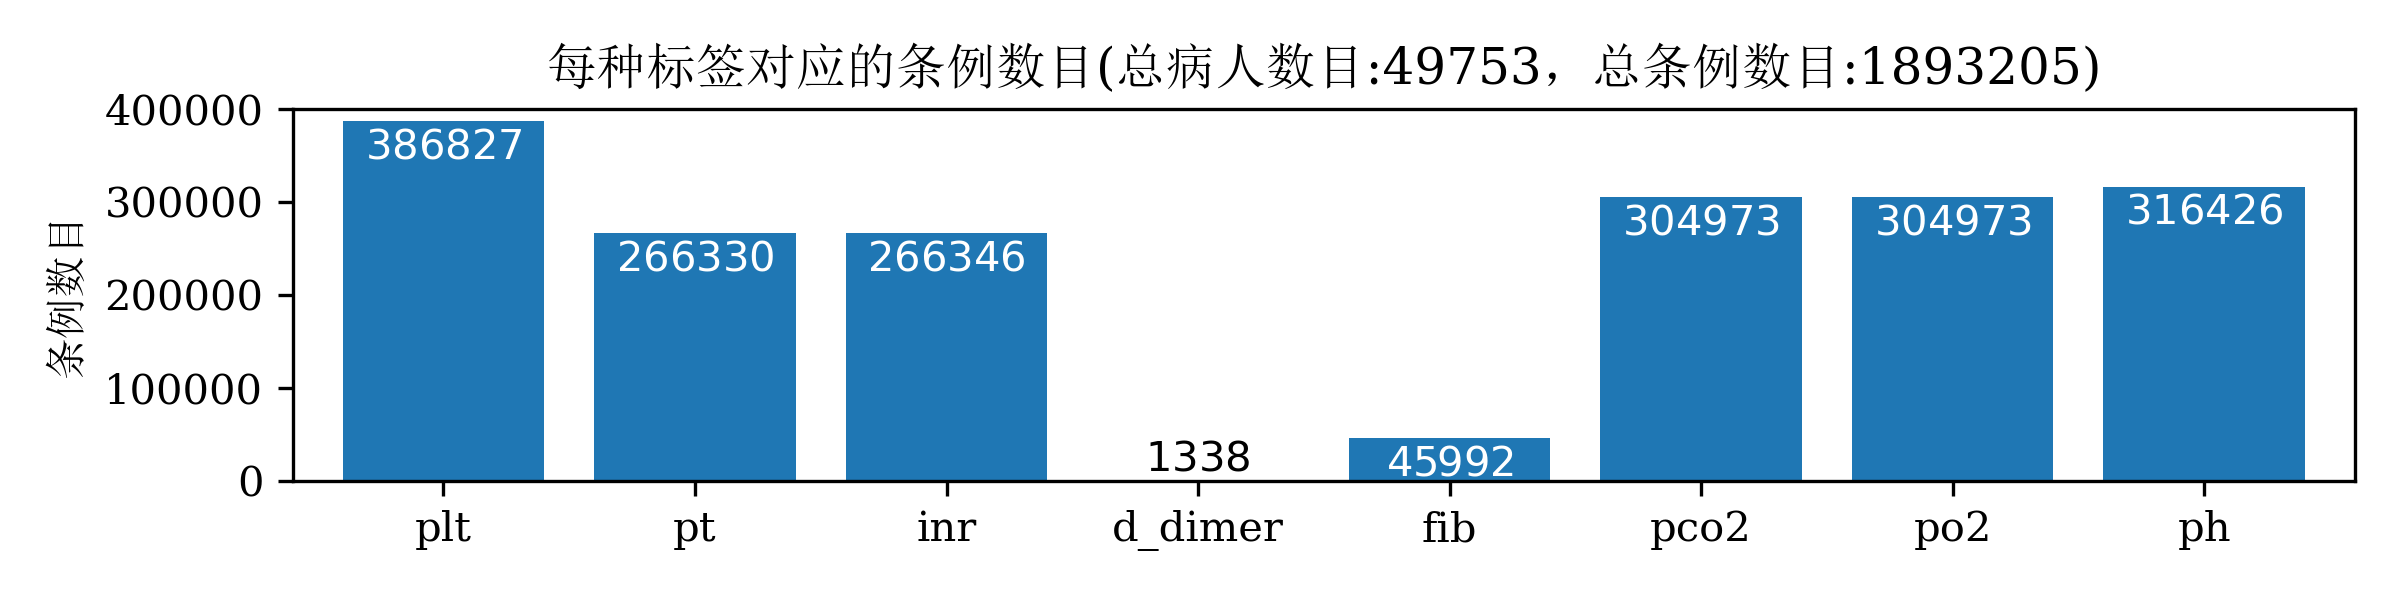
\includegraphics[scale=0.21]{labels_vs_total_number_plot.png}
       % \caption{DIC重要度排名(基于随机森林)}
   \end{subfigure}
   
   %\bigskip
   \begin{subfigure}{0.9\textwidth}
       \hspace{-1.5cm}
       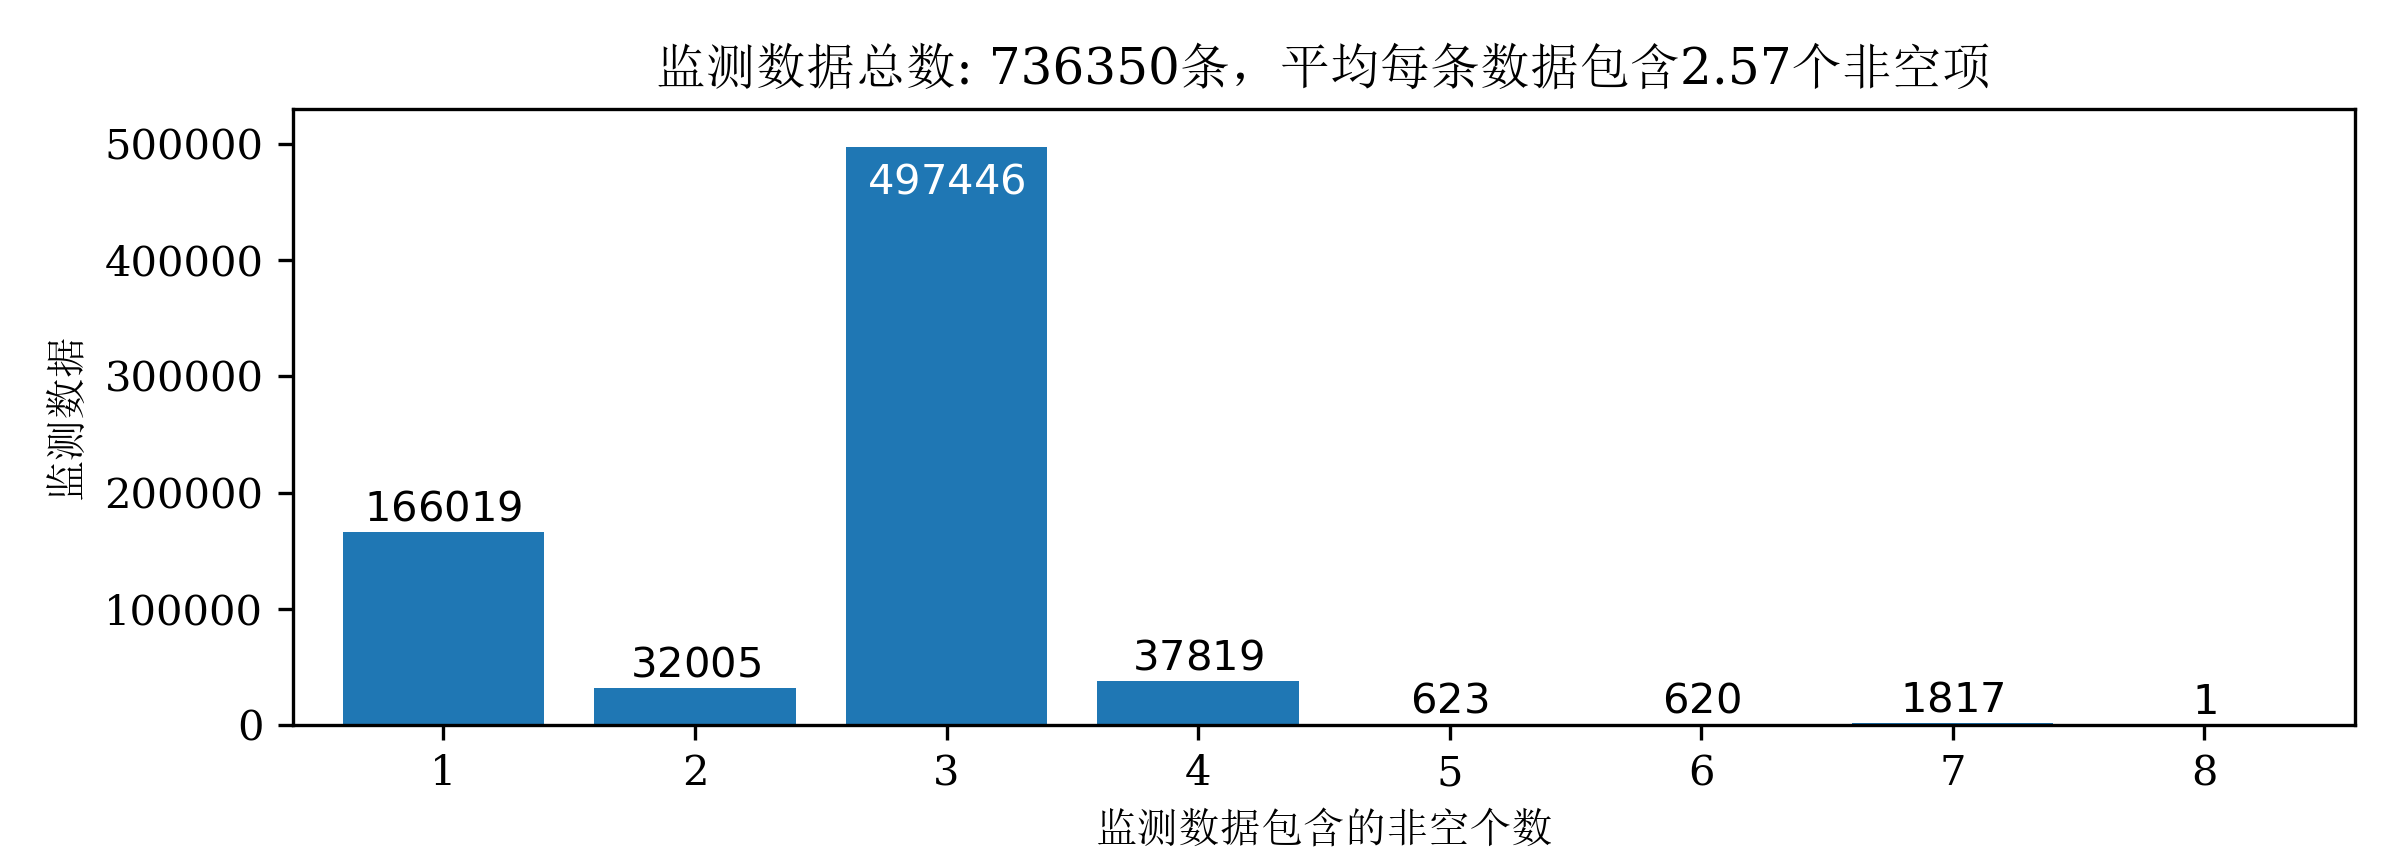
\includegraphics[scale=0.2105]{not_null_num_vs_monitor_data_plot}
       % \caption{}
   \end{subfigure}
   \caption{数据提取结果}
   \label{fig-capture}
\end{figure}
\subsubsection{数据插补}
进行数据插补前,我们首先要以某个起始时刻$T_0$作为基准时间,其他时刻均对$T_0$做差,并转化为小时为单位的时间,
具体实现如算法\ref{alg-time}所示。
\begin{algorithm}[H]
    \caption{时间转换}\label{alg-time}
    \begin{pythoncode}
charttimes = df['charttime']
# 以最小时间戳 charttimes.min() 作为基准时间,计算其他时间与其的相对时间差
time_format = '%Y-%m-%d %H:%M:%S'
base_time = datetime.strptime(charttimes.min(), time_format)

# 计算与基准时间的相对时间差(单位:小时,浮点型)
def relative_hours(date_string): 
    date = datetime.strptime(date_string, time_format)
    relative_days = (date - base_time).days  # 相对天数
    relative_seconds = (date - base_time).seconds  # 相对秒数
    relative_hours = 24 * relative_days + relative_seconds / 3600
    return relative_hours
    \end{pythoncode}
\end{algorithm}
\vspace{-1em}
数据插补的方法就是将同一个病人在同一时间段内的信息进行合并,从而得到一个时间段内的数据整体作为新的数据集。
我们记时间段长度为$L$小时,例如当$L=8$时,说明需要将两个相邻时间小于等于$8$小时的数据进行合并。

设当前病人具有$N$条信息,将第$i\in\{1,\cdots,N\}$条信息记为$\bd{x}^{(i)} = \{x_k^{(i)}\}_{k=1}^8\in \R^8$,该信息的相对时间为$t_i$;
设第$j$个时间段为$[T_j,T_j+8)$,其对应的特征向量为$\bd{y}^{(i)} = \{y_k^{(i)}\}_{k=1}^8\in\R^8$。 我们设计了以下两种插补方法:
\paragraph{覆盖插补}使用该时间段中的最后一次非空特征值做插补:
\begin{equation}
    y_k^{(j)}\gets x_k^{(i)},\quad s.t.\begin{cases}
        t_i = \max_{t_i\in[T_j,T_j+L)}t_i,\\
        x_k^{(i)}\ \text{非空}.
    \end{cases}
\end{equation}
\paragraph{均值插补}若该时间段中存在对于第$k\in[1,8]$个特征有多条信息,则取均值做插补:
\begin{equation}
    y_k^{(i)}\gets\frac{1}{N_k^{(i)}}\sum_{\substack{t_i\in[T_j,T_j+8)\\ x_k^{(i)}\ \text{非空}}}x_k^{(j)}
\end{equation}
其中$N_k^{(i)} = \#\{t_i:t_i\in[T_j,T_j+8), x_k^{(i)}\ \text{非空}\}$,$\#S$表示集合$S$的基数。
\renewcommand\arraystretch{1.2} % 设置表格高度为原来的0.8倍
\begin{table}[H] % table标准
    \centering % 表格居中
    \begin{tabular}{p{0.3\textwidth}<{\centering}p{0.6\textwidth}} % 设置表格宽度
    %\begin{tabular}{cccc}
        \toprule
        \textbf{符号}&\textbf{意义}(以下定义中的信息均来自同一个病人)\\
        \midrule
        $x_{time}^{(i)}$&\textbf{时间戳:}第$i$个信息$\bd{x}^{(i)}$对应的时刻\\
        $S=(\bd{x}^{(i_1)},\cdots,\bd{x}^{(i_k)})$&\textbf{信息段:}\makecell[l]{按照信息的时间戳从小大大排序,\\
        并且满足$x_{time}^{(i_k)}-x_{time}^{(i_1)}\leq L$}\\
        $S_1\prec S_2$&\textbf{信息段的序关系:}\makecell[l]{$\bd{x}_{time}<\bd{y}_{time},(\bd{x}\in S_1,\bd{y}\in S_2)$}\\
        $S_1\sim S_2$&\textbf{连续信息段:}\makecell[l]{$\min_{\bd{y}\in S_2}y_{time} - \max_{\bd{x}\in S_1}x_{time}\leq L,(S_1\prec S_2)$}\\
        $S_1\sim S_2\sim\cdots\sim S_k$&\textbf{多个连续信息段:}$S_i\sim S_{i+1},(i=1,\cdots,k-1)$\\
        $B = \{S_1,S_2\cdots,S_k\}$&\textbf{信息块:}$S_1\sim\cdots\sim S_k$且$k\geq 2$\\
        \bottomrule
    \end{tabular}
    \caption{符号定义}
    \label{table-define}
\end{table}

为更清晰的描述插补后的数据,我们给出如表\ref{table-define}中对信息段与信息块的定义,上述定义说明:同一病人
的任意两个信息段$S_i,S_j,(i\neq j)$均有序关系成立,并且信息块$B$是由至少两个连续信息段构成的。

我们之所以要这样定义信息块,是因为首先要保证其中的信息段之间的时间差不超过$L$小时,这样才能使得新的数据信息具有时序性,
并且要求信息段至少有两个,因为我们希望通过前几个连续的时间段预测未来的一个时间段是否会患有DIC.
 
数据插补得到的最终结果为每个病人的全部信息块,经过插补操作后每种表情对应的非空信息占比如图\ref{fig-interpolation}
\vspace{-1em}
\begin{figure}[H]
    \hspace{-1.5cm}
    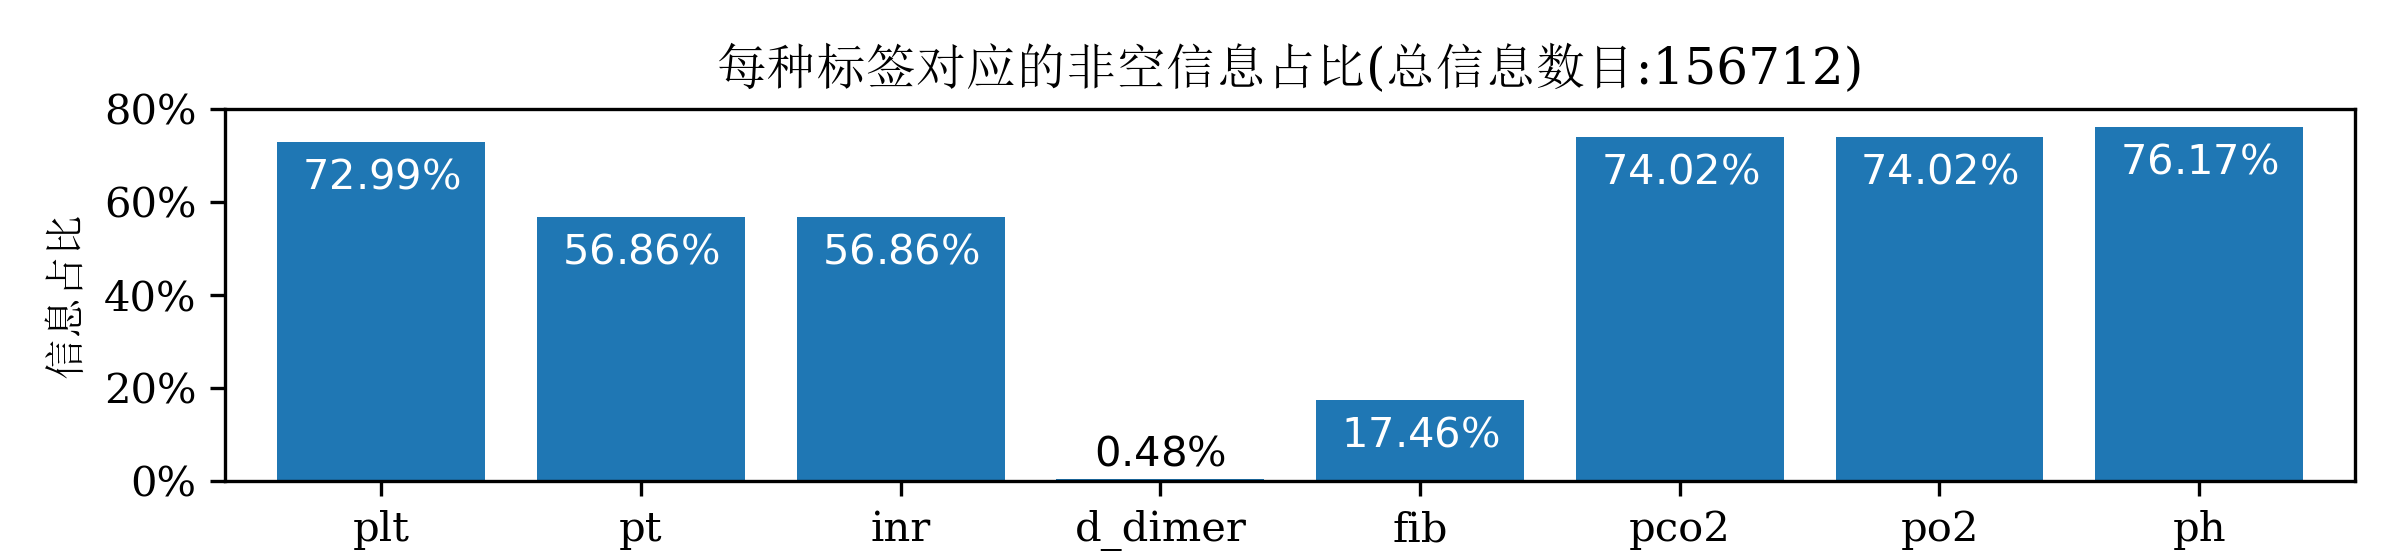
\includegraphics[scale=0.21]{info_vs_ratio_label_plot}
    \caption{插补操作后非空信息占比}
    \label{fig-interpolation}
\end{figure}
\subsubsection{异常值矫正}
我们按照表\ref{table-limit}中定义的极限范围对数据进行异常值矫正,即若数据超过极大范围则调整至最大极限值,反之亦然。
\renewcommand\arraystretch{1.2} % 设置表格高度为原来的1.2倍
\begin{table}[H] % table标准
    \centering % 表格居中
    \begin{tabular}{p{0.23\textwidth}p{0.12\textwidth}p{0.2\textwidth}<{\centering}
        p{0.2\textwidth}<{\centering}p{0.1\textwidth}} % 设置表格宽度
        \toprule
        \textbf{名称}&\textbf{缩写}&\textbf{正常范围}&\textbf{极限范围}&\textbf{单位}\\
        \midrule
        血小板计数&\texttt{plt}&$[100,300]$&$[10,300]$&$\times 10^9/\text{L}$\\
        凝血原酶时间&\texttt{pt}&$\leq 16$&$[7,30]$&$s$(秒)\\
        国际标准化比值&\texttt{inr}&$[0.8,1.4]$&$[0.5,2]$&无\\
        D-二聚体&\texttt{d\_dimer}&$500$左右&$[100,10000]$&$\text{ug}/\text{L}$\\
        纤维蛋白原&\texttt{fib}&$[1000,2000]$&$[10,2000]$&$\text{mg}/\text{L}$\\
        二氧化碳分压&\texttt{pco2}&$[35,45]$&$[5,250]$&$\text{mmHg}$\\
        氧分压&\texttt{po2}&$[80,100]$&$[20,500]$&$\text{mmHg}$\\
        酸碱度&\texttt{ph}&$[7.35,7.45]$&$[6,8]$&无\\
        \bottomrule
    \end{tabular}
    \caption{每类数据的极限范围及对应单位}
    \label{table-limit}
\end{table}
\subsubsection{数据填补}
从图\ref{fig-interpolation}中可以看出,经过插补后的数据中\texttt{fib}偏少,而\texttt{d\_dimer}极少,
我们尝试了一下三种方法对缺失数据进行填补。
\paragraph{均值填补}若一个信息块$B$中的某个信息段$s\in B$的第$k$维属性值为空,分以下两种情况:
\begin{itemize}
    \item 若存在该信息块中其他信息段该属性值非空,则使用该属性的其他非空值的均值进行填补:
    \begin{equation*}
        s_k\gets \frac{1}{\#\{s:s\in B,s_k\ \text{非空}\}}\sum_{s\in B, s_k\ \text{非空}}s_k
    \end{equation*}
    \item 若该信息块中$k$维属性值全部为空,则直接用正常值进行填补,每种属性的正常值取表\ref{table-limit}中
    正常范围的中位数。
\end{itemize}
\paragraph{自适应多项式填补策略}
考虑到一个信息块中的各项属性之在每个时间段下不会是恒定值,于是我们在以上策略的基础上引入自适应多项式填补策略,
假设信息块$S$中第$k$维属性值有$m$个非空值,分为一下三种情况:
\begin{itemize}
    \item $m=0$,全部为空值,则全部使用正常值进行填补。
    \item $m=1$,仅有一个数据,则全部使用该数据进行填充。
    \item $m>1$,使用$[m/2]$阶多项式对空值进行回归预测。($[x]$表示对实数$x$向下取整)
\end{itemize}
假设回归数据中$x$为对应的非空值,先进行多项式特征提取转化为线性回归问题(若多项式阶数$n=3$,则提取出$x^3,x^2,x^1,1$项),
然后进行标准化处理,再使用SVD分解求解最小二乘回归问题,最后将多项式模型对空值的索引进行插值,得到对应的预测结果。
\paragraph{基于24小时有效范围的临近填补}
考虑到一个信息块$B$中的内容如果使用较长时间差的点进行填补则会出现较大的误差,并且如果使用高阶多项式进行拟合可能出现Runge现象
(如图\ref{fig-imputer}所示),
所以我们基于上面两个方法提出一种简单易行的且更符合现实的填补方法:

考虑使用24小时内的非空信息对空信息进行填补,对于一个信息块中空信息,
我们取24小时内与之最接近的数据信息对其进行填补,若没有任何24小时内的数据,则抛弃该信息。
\vspace{-1em}
\begin{figure}[H]
   \hspace{-1cm}
   % 如果一行放三个图改成0.3\linewidth即可
   \begin{subfigure}[b]{0.55\textwidth}
       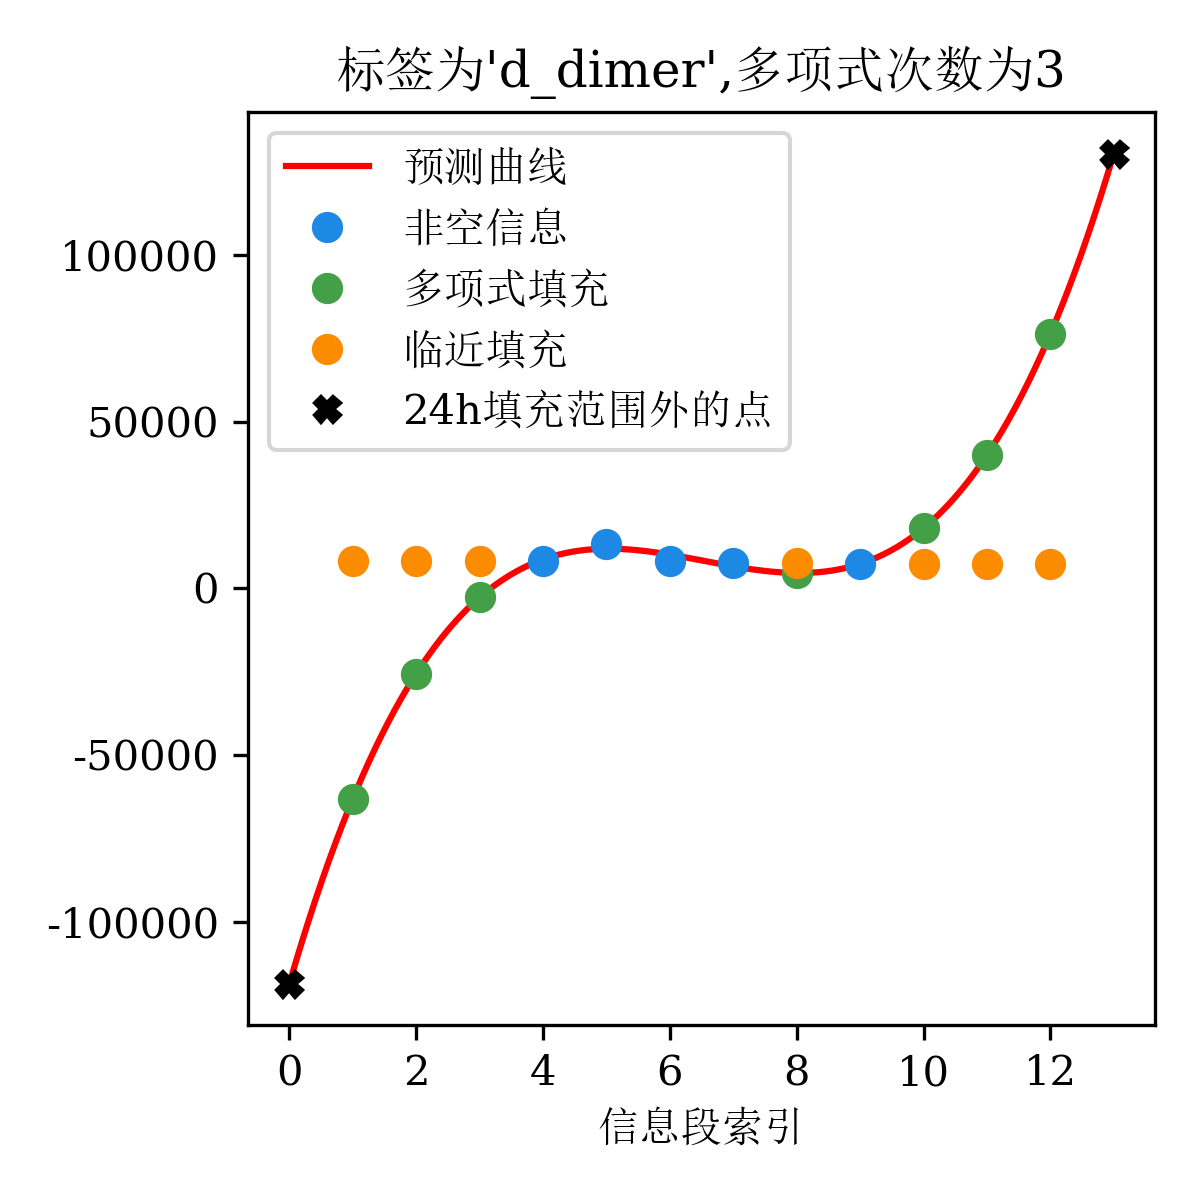
\includegraphics[scale=0.2]{polynomial_neighbor_imputer_24hours_plot0}
       \caption{第36534个信息块}
   \end{subfigure}
   \begin{subfigure}[b]{0.6\textwidth}
       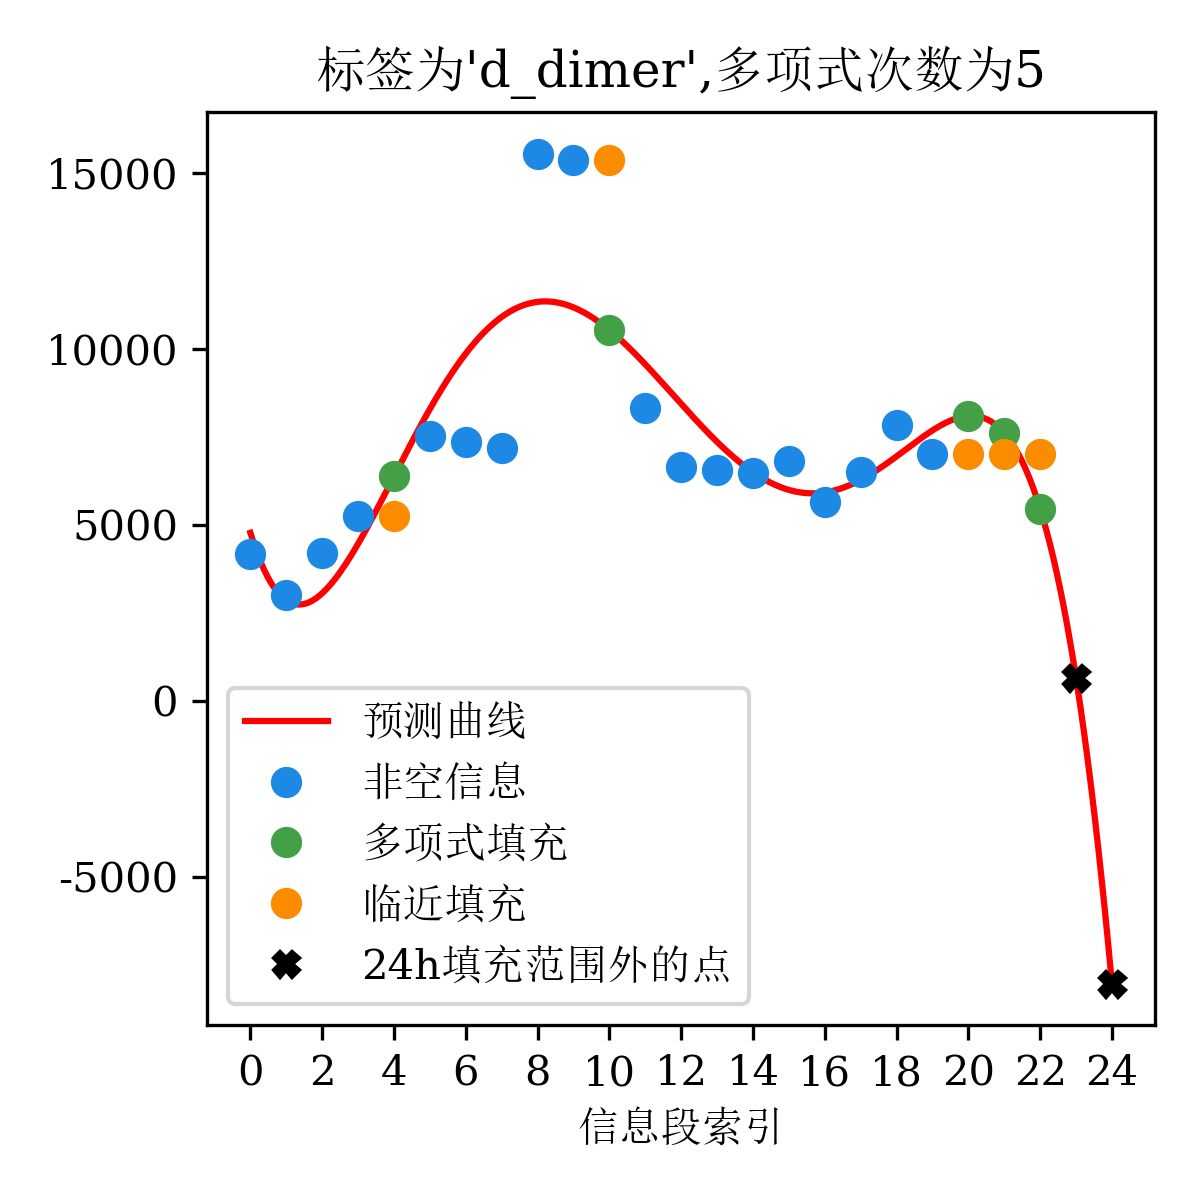
\includegraphics[scale=0.2]{polynomial_neighbor_imputer_24hours_plot1}
       \caption{第13032个信息块}
       \label{fig-regular}
   \end{subfigure}
   \caption{不同填充方法比较}
   \label{fig-imputer}
\end{figure}

图\ref{fig-imputer}中,红色曲线为多项式预测曲线,左右两段的黑色标记点表明时间超过了24小时,并且可以看出多项式填补的数据严重偏离
非空值,这种问题可能是由于过拟合导致,我们尝试加入正则项进行改进,得到如图\ref{fig-regular}所示,
从该图中看出填补效果仍然不好,所以最终舍弃了该填补方法。
图\ref{fig-imputer-null-compare}显示了经过填补操作后每个信息中包含的非空数据量有明显增加。
\begin{figure}[htbp]
    \vspace{-1em}
    \hspace{-1.4cm}
    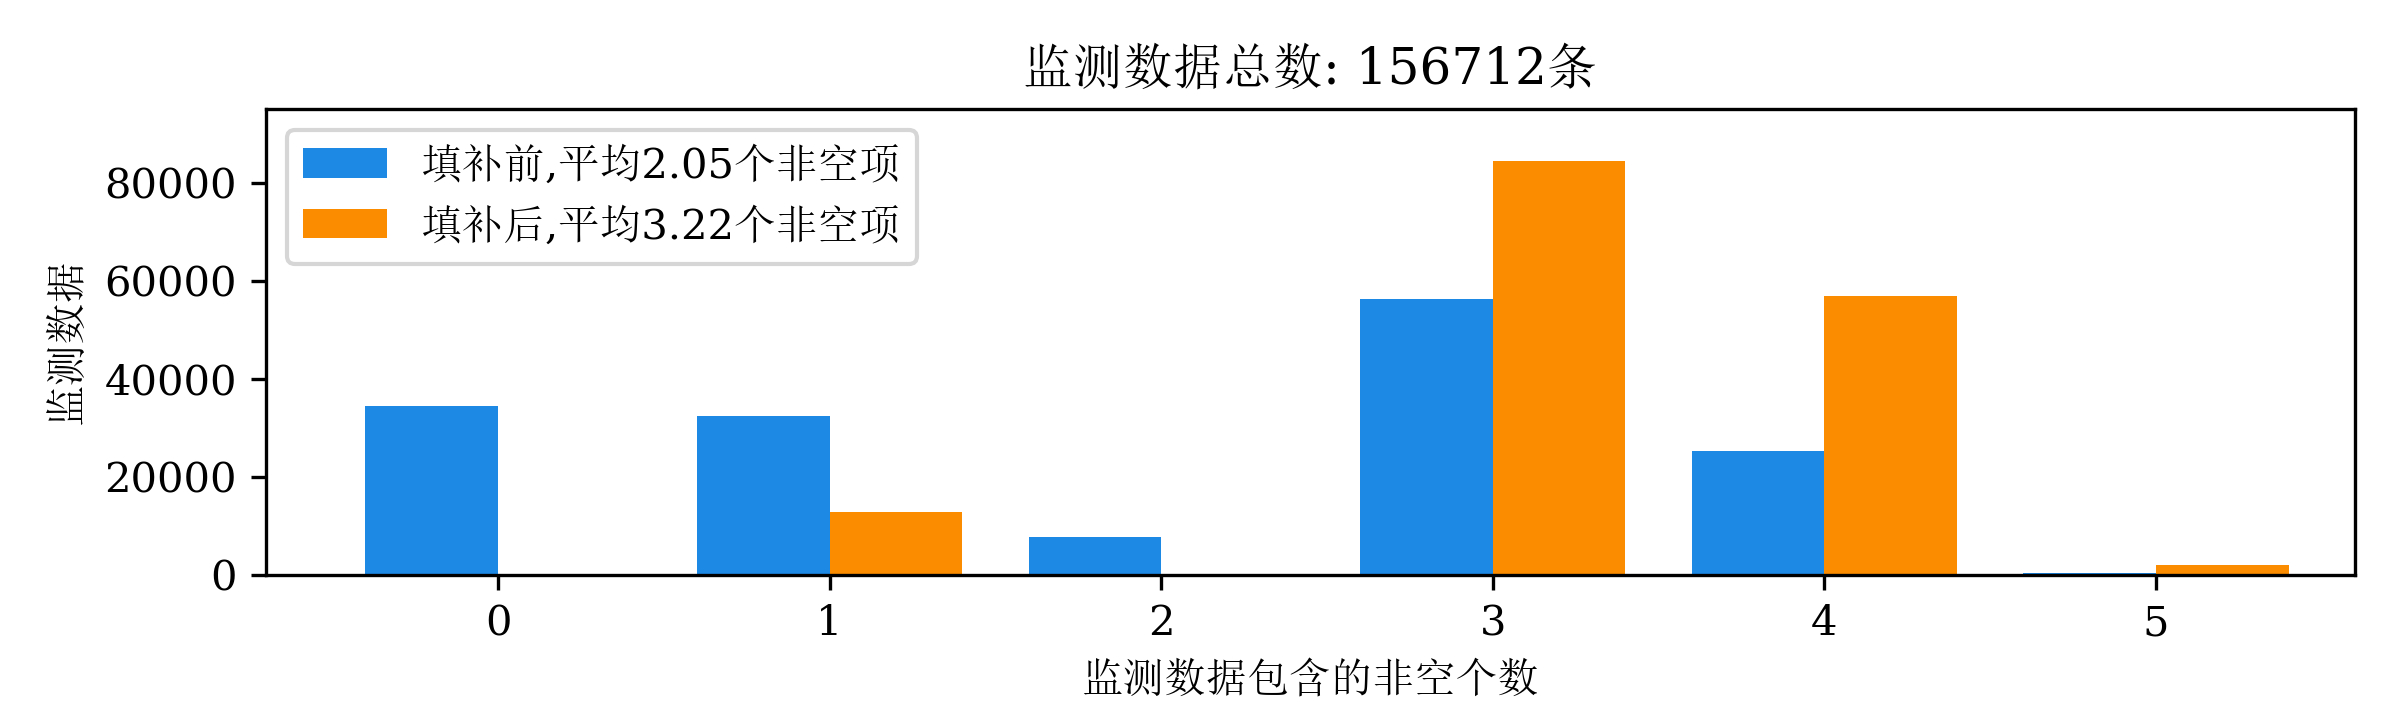
\includegraphics[scale=0.21]{before_vs_after_impute_null_data_number_plot}
    \caption{填补前后的非空值对比}
    \label{fig-imputer-null-compare}
\end{figure}
\subsubsection{实时状态数据标记}
根据文献\cite{bib-determine-dic}中给出的标记指标,我们可以结合SIC评分和ISTH显性DIC评分来对病人每个时刻是否可能患有脓毒症进行标记,
具体标注规则如表\ref{table-label}所示:
\renewcommand\arraystretch{1.2} % 设置表格高度为原来的1.2倍
\begin{table}[H] % table标准
    \centering % 表格居中
\begin{tabular}{ccllccl}
\cline{1-3} \cline{5-7}
\multicolumn{1}{|c|}{指标}                   & \multicolumn{1}{c|}{评分} & \multicolumn{1}{c|}{SIC评分标准}      & \multicolumn{1}{c|}{} & \multicolumn{1}{c|}{指标}                       & \multicolumn{1}{c|}{评分} & \multicolumn{1}{c|}{DIC评分标准}        \\ \cline{1-3} \cline{5-7} 
\multicolumn{1}{|c|}{\multirow{3}{*}{PLT}} & \multicolumn{1}{c|}{2}  & \multicolumn{1}{l|}{(0, 100)}     & \multicolumn{1}{l|}{} & \multicolumn{1}{c|}{\multirow{3}{*}{PLT}}     & \multicolumn{1}{c|}{2}  & \multicolumn{1}{l|}{(0, 50)}        \\ \cline{2-3} \cline{6-7} 
\multicolumn{1}{|c|}{}                     & \multicolumn{1}{c|}{1}  & \multicolumn{1}{l|}{{[}100, 150)} & \multicolumn{1}{l|}{} & \multicolumn{1}{c|}{}                         & \multicolumn{1}{c|}{1}  & \multicolumn{1}{l|}{{[}50, 100)}    \\ \cline{2-3} \cline{6-7} 
\multicolumn{1}{|c|}{}                     & \multicolumn{1}{c|}{0}  & \multicolumn{1}{l|}{{[}150, $\infty$)}   & \multicolumn{1}{l|}{} & \multicolumn{1}{c|}{}                         & \multicolumn{1}{c|}{0}  & \multicolumn{1}{l|}{{[}100, $\infty$)}     \\ \cline{1-3} \cline{5-7} 
\multicolumn{1}{|c|}{\multirow{3}{*}{INR}} & \multicolumn{1}{c|}{2}  & \multicolumn{1}{l|}{(1.4, $\infty$)}     & \multicolumn{1}{l|}{} & \multicolumn{1}{c|}{\multirow{3}{*}{D-Dimer}} & \multicolumn{1}{c|}{3}  & \multicolumn{1}{l|}{{[}7000, $\infty$)}    \\ \cline{2-3} \cline{6-7} 
\multicolumn{1}{|c|}{}                     & \multicolumn{1}{c|}{1}  & \multicolumn{1}{l|}{(1.2, 1.4{]}} & \multicolumn{1}{l|}{} & \multicolumn{1}{c|}{}                         & \multicolumn{1}{c|}{2}  & \multicolumn{1}{l|}{{[}3000, 7000)} \\ \cline{2-3} \cline{6-7} 
\multicolumn{1}{|c|}{}                     & \multicolumn{1}{c|}{0}  & \multicolumn{1}{l|}{(0, 1.2{]}}   & \multicolumn{1}{l|}{} & \multicolumn{1}{c|}{}                         & \multicolumn{1}{c|}{0}  & \multicolumn{1}{l|}{(0, 3000)}      \\ \cline{1-3} \cline{5-7} 
\multicolumn{3}{c}{\multirow{2}{*}{\makecell{当SIC总分$\geq 2$时,\\标记为SIC个体}}}                                                  & \multicolumn{1}{l|}{} & \multicolumn{1}{c|}{\multirow{2}{*}{FIB}}     & \multicolumn{1}{c|}{1}  & \multicolumn{1}{l|}{(0,1000)}       \\ \cline{6-7} 
\multicolumn{3}{c}{}                                                                                     & \multicolumn{1}{l|}{} & \multicolumn{1}{c|}{}                         & \multicolumn{1}{c|}{0}  & \multicolumn{1}{l|}{{[}1000, $\infty$)}    \\ \cline{5-7} 
\multicolumn{1}{l}{}                       & \multicolumn{1}{l}{}    &                                   & \multicolumn{1}{l|}{} & \multicolumn{1}{c|}{\multirow{3}{*}{PT}}      & \multicolumn{1}{c|}{2}  & \multicolumn{1}{l|}{{[}19, $\infty$)}      \\ \cline{6-7} 
\multicolumn{1}{l}{}                       & \multicolumn{1}{l}{}    &                                   & \multicolumn{1}{l|}{} & \multicolumn{1}{c|}{}                         & \multicolumn{1}{c|}{1}  & \multicolumn{1}{l|}{{[}16, 19)}     \\ \cline{6-7} 
\multicolumn{1}{l}{}                       & \multicolumn{1}{l}{}    &                                   & \multicolumn{1}{l|}{} & \multicolumn{1}{c|}{}                         & \multicolumn{1}{c|}{0}  & \multicolumn{1}{l|}{{[}0, 16)}      \\ \cline{5-7} 
\multicolumn{1}{l}{}                       & \multicolumn{1}{l}{}    &                                   &                       & \multicolumn{3}{c}{\multirow{2}{*}{\makecell{当标记为SIC个体,且DIC总分$\geq 4$时,\\标记为DIC个体}}}                                             \\
\multicolumn{1}{l}{}                       & \multicolumn{1}{l}{}    &                                   &                       & \multicolumn{3}{c}{}                                                                                         
\end{tabular}
    \caption{SIC与DIC标注规则}
    \label{table-label}
\end{table}

使用上述填补数据进行标记后,得到的不同时间段下SIC和DIC信息占比结果由附录中表\ref{table-sic-dic}所示。

\clearpage
\section{模型训练与评估}
\subsection{数据集划分}
首先需要将数据集划分为训练集与测试集,设$N_t$为序列长度,我们期望用前$N_t$个信息段的信息预测后一个信息段是否患病,
设信息块为$B = (\bd{s}^{(1)}, \bd{s}^{(2)},\cdots,\bd{s}^{(n)})$,将$N_t+1$个时间段视为一个\textbf{时间窗口},于是由$B$
生成的时间窗口可以表示为
\begin{equation*}
    \{(\bd{s}^{(k)},\bd{s}^{(k+1)},\cdots,\bd{s}^{(k+N_t)}):1\leq k\leq n-N_t\}
\end{equation*}
总计$n-N_t$个时间窗口,记信息$\bd{s}^{(k)}$包含$8$个维度的特征为$\bd{s}_x^{(k)}$,将其对应的标记为$\bd{s}_{label}^{(k)}$
(如果是预测DIC,则标记表示第$k$个信息段中是否被标记为DIC,预测SIC同理),
于是一个时间窗口就可以构造出如下的一组数据:
\begin{equation*}
    \begin{cases}
        \bd{x} = \left(\bd{s}_x^{(k)},\bd{s}_x^{(k+1)},\cdots,\bd{s}_x^{(k+N_t-1)}\right)\in \R^{8\times N_{t}},\add\\
        y = \bd{s}_{label}^{(k+N_t)}.
    \end{cases}
\end{equation*}
最后我们将数据集按照$4:1$\textbf{按标签比例分层抽样},划分为训练集与测试集,数据集划分结果见附录表\ref{table-divide}。
\subsection{模型评估}
由于本训练集最终得到的数据量较小,所以考虑使用传统机器学习方法,我们尝试了以下5中算法:使用随机梯度下降优化的线性模型(SGD)、
SVM模型、决策树、随机森林、K近邻。并采取了以下三个评估指标对:
\begin{itemize}
    \item 在训练集上使用K-折叠交叉验证模型准确率。
    \item 在测试集上的准确率。
    \item ROC曲线下面积(AUC)。
\end{itemize}
我们通过在模型在测试集上的准确率(附录表\ref{table-ML-compare})来对数据集的参数进行选取,对于DIC指标,
我们发现在序列长度为$2$、时间段长度为4h时,模型准确率较高;对于SIC指标,综合考虑我们发现在序列长度为$3$、时间段长度为8h时,
效果较好,其他在$98\%$以上的结果我们认为是数据量较少导致的。

接下来我们在各自的最优数据集上使用K-折交叉验证和AUC分别进一步筛选DIC模型和SIC模型,结果如表\ref{table-dic},\ref{table-sic}所示。
并在图\ref{fig-ML-compare}中的分别展示了完整的ROC曲线,同时给出了基于随机森林的特征重要度分布。
%\renewcommand\arraystretch{1.2} % 设置表格高度为原来的1.2倍
\vspace{-0.5em}
\begin{table}[H] % table标准
    \centering % 表格居中
\begin{tabular}{clcc}
    \toprule
\textbf{模型名称} & \textbf{K-折交叉验证准确率}        & \textbf{测试集准确率} & \textbf{ROC\_AUC} \\
    \midrule
SGD           & {[}0.9151 0.8774 0.8396{]} & 0.9125          & 0.9497            \\
SVC           & {[}0.934  0.9057 0.9245{]} & 0.9625          & 0.956             \\
决策树           & {[}0.8774 0.9057 0.8774{]} & 0.9875          & 0.8399            \\
随机森林          & {[}0.9245 0.9434 0.9151{]} & 0.9875          & 0.9671            \\
KNN           & {[}0.9057 0.9245 0.8962{]} & 0.95            & 0.9252           \\
    \bottomrule
\end{tabular}
    \caption{DIC模型选择}
    \label{table-dic}
\end{table}

\begin{table}[H] % table标准
    \centering % 表格居中
\begin{tabular}{clcc}
    \toprule
\textbf{模型名称} & \textbf{K-折交叉验证准确率}        & \textbf{测试集准确率} & \textbf{ROC\_AUC} \\
    \midrule
SGD           & {[}0.943  0.9534 0.9482{]} & 0.9655          & 0.9599            \\
SVC           & {[}0.9326 0.9585 0.9326{]} & 0.9586          & 0.9641            \\
决策树           & {[}0.943  0.9482 0.9223{]} & 0.9448          & 0.8374            \\
随机森林          & {[}0.9482 0.943  0.9275{]} & 0.9793          & 0.973             \\
KNN           & {[}0.9223 0.943  0.9482{]} & 0.9379          & 0.9171           \\
    \bottomrule
\end{tabular}
    \caption{SIC模型选择}
    \label{table-sic}
\end{table}
\begin{figure}[htbp]
    \hspace{-2cm}
    % 如果一行放三个图改成0.3\linewidth即可
    \begin{subfigure}[b]{0.6\textwidth}
        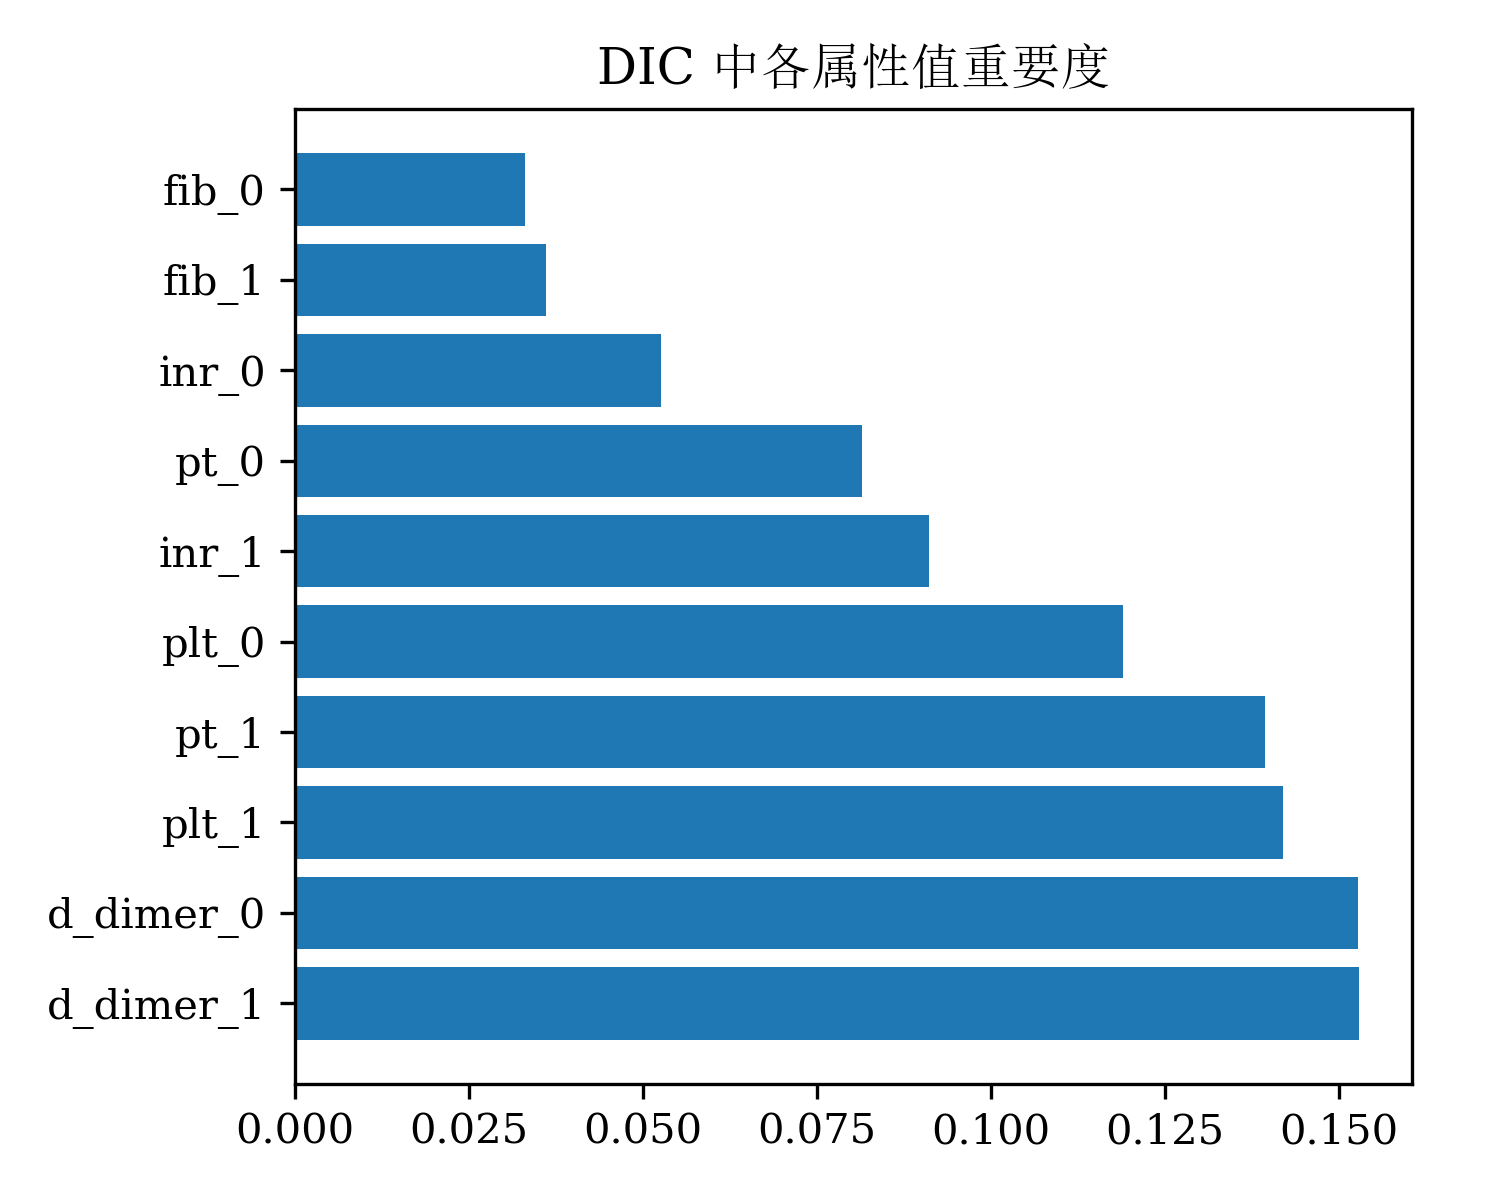
\includegraphics[scale=0.75]{dic_attributes_rank.png}
        \caption{DIC重要度排名(基于随机森林)}
    \end{subfigure}
    \begin{subfigure}[b]{0.6\textwidth}
        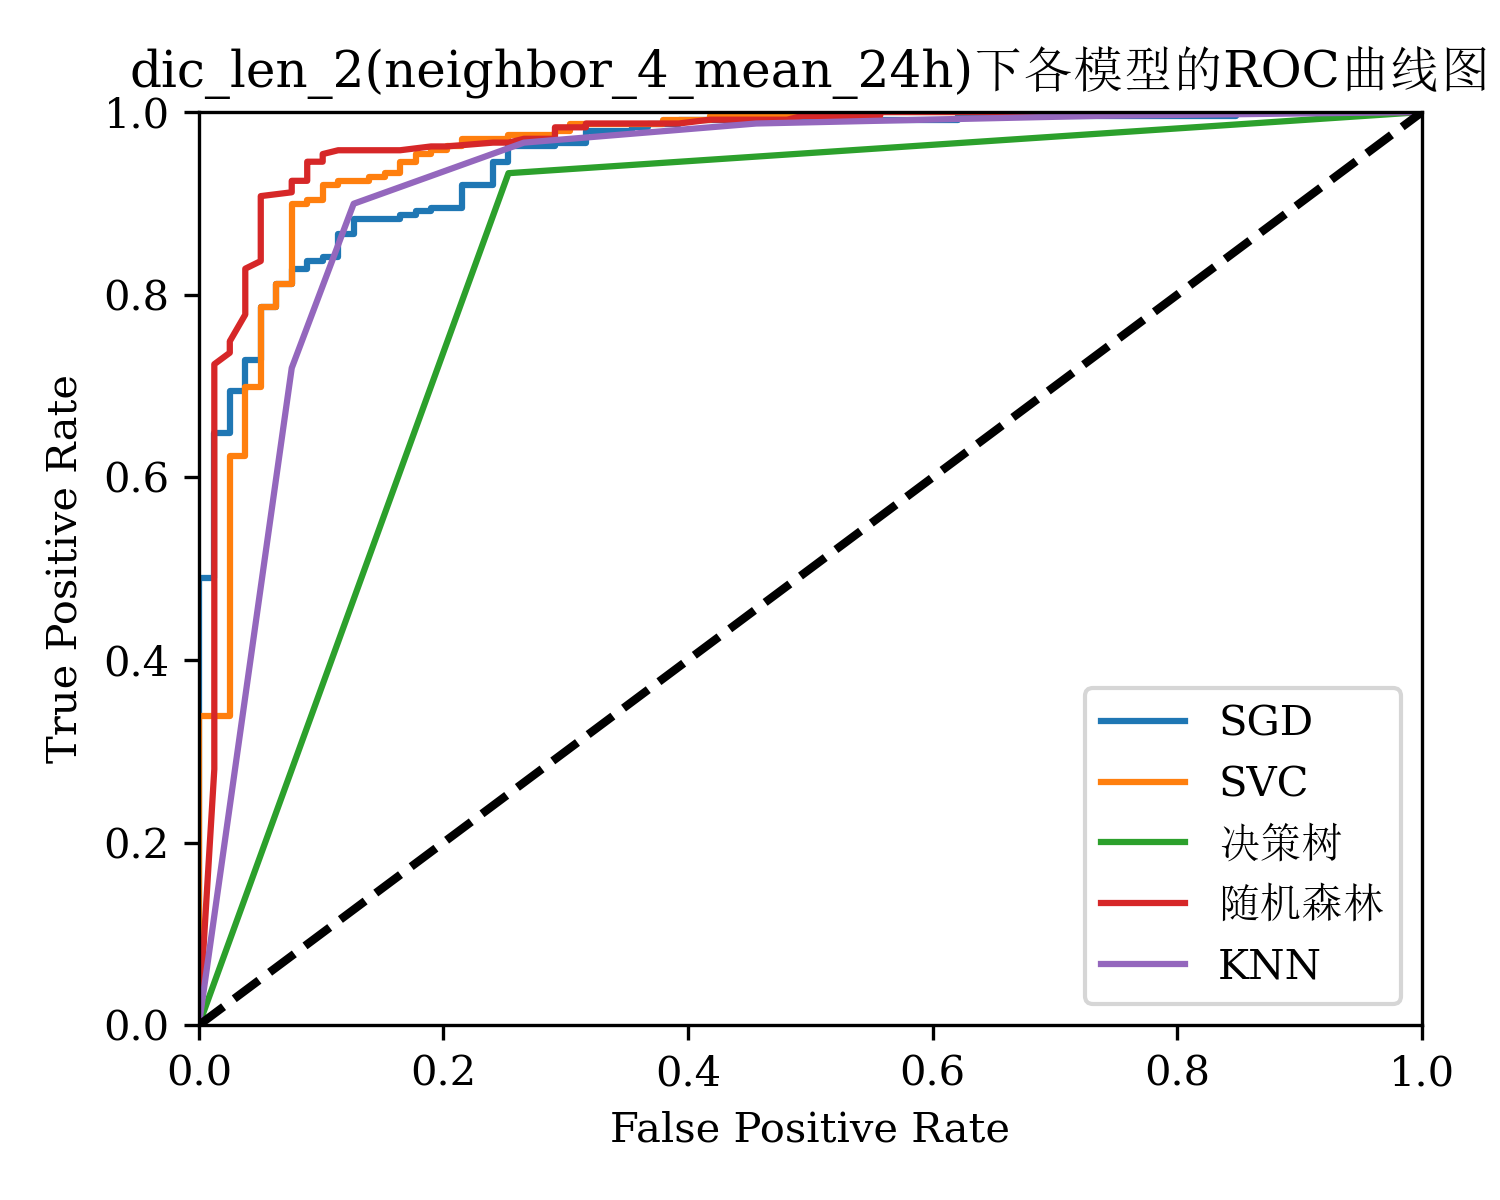
\includegraphics[scale=0.75]{dic_len_2(neighbor_4_mean_24h)_roc_curves.png}
        \caption{不同模型对DIC预测的ROC值}
    \end{subfigure}
    
    \bigskip
    \hspace{-2cm}
    \begin{subfigure}{0.6\textwidth}
        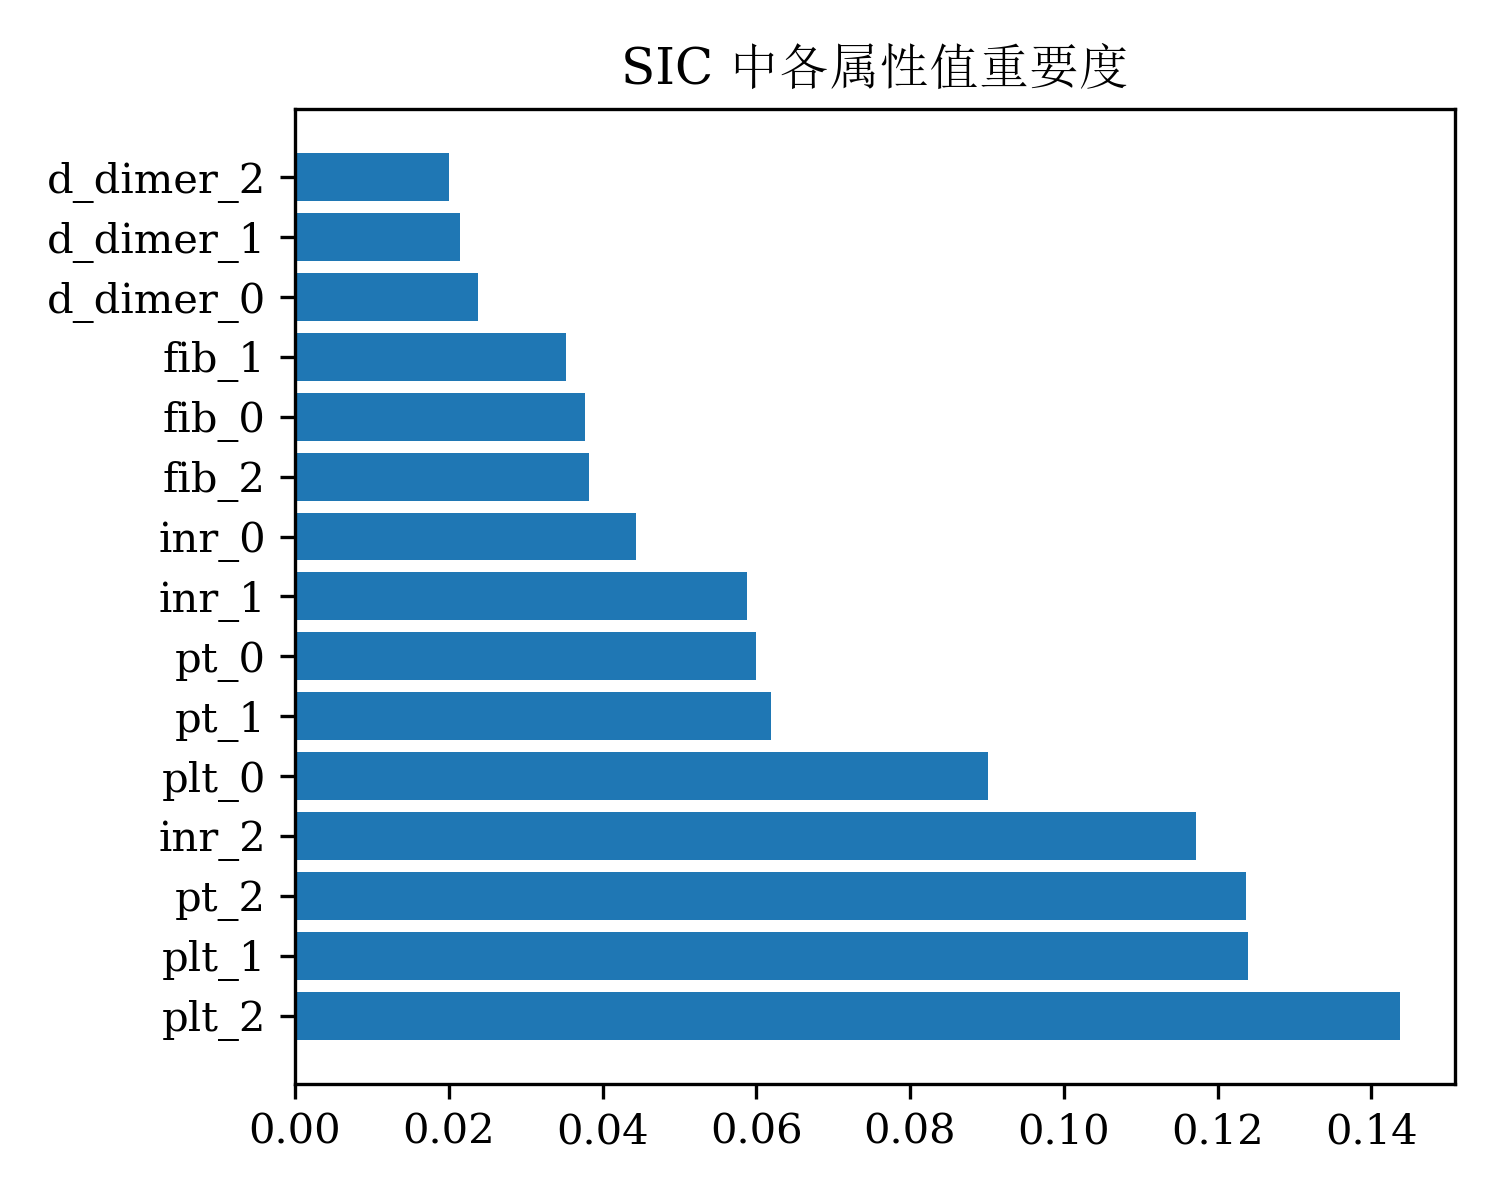
\includegraphics[scale=0.75]{sic_attributes_rank.png}
        \caption{SIC重要度排名(基于随机森林)}
    \end{subfigure}
    \begin{subfigure}{0.6\textwidth}
        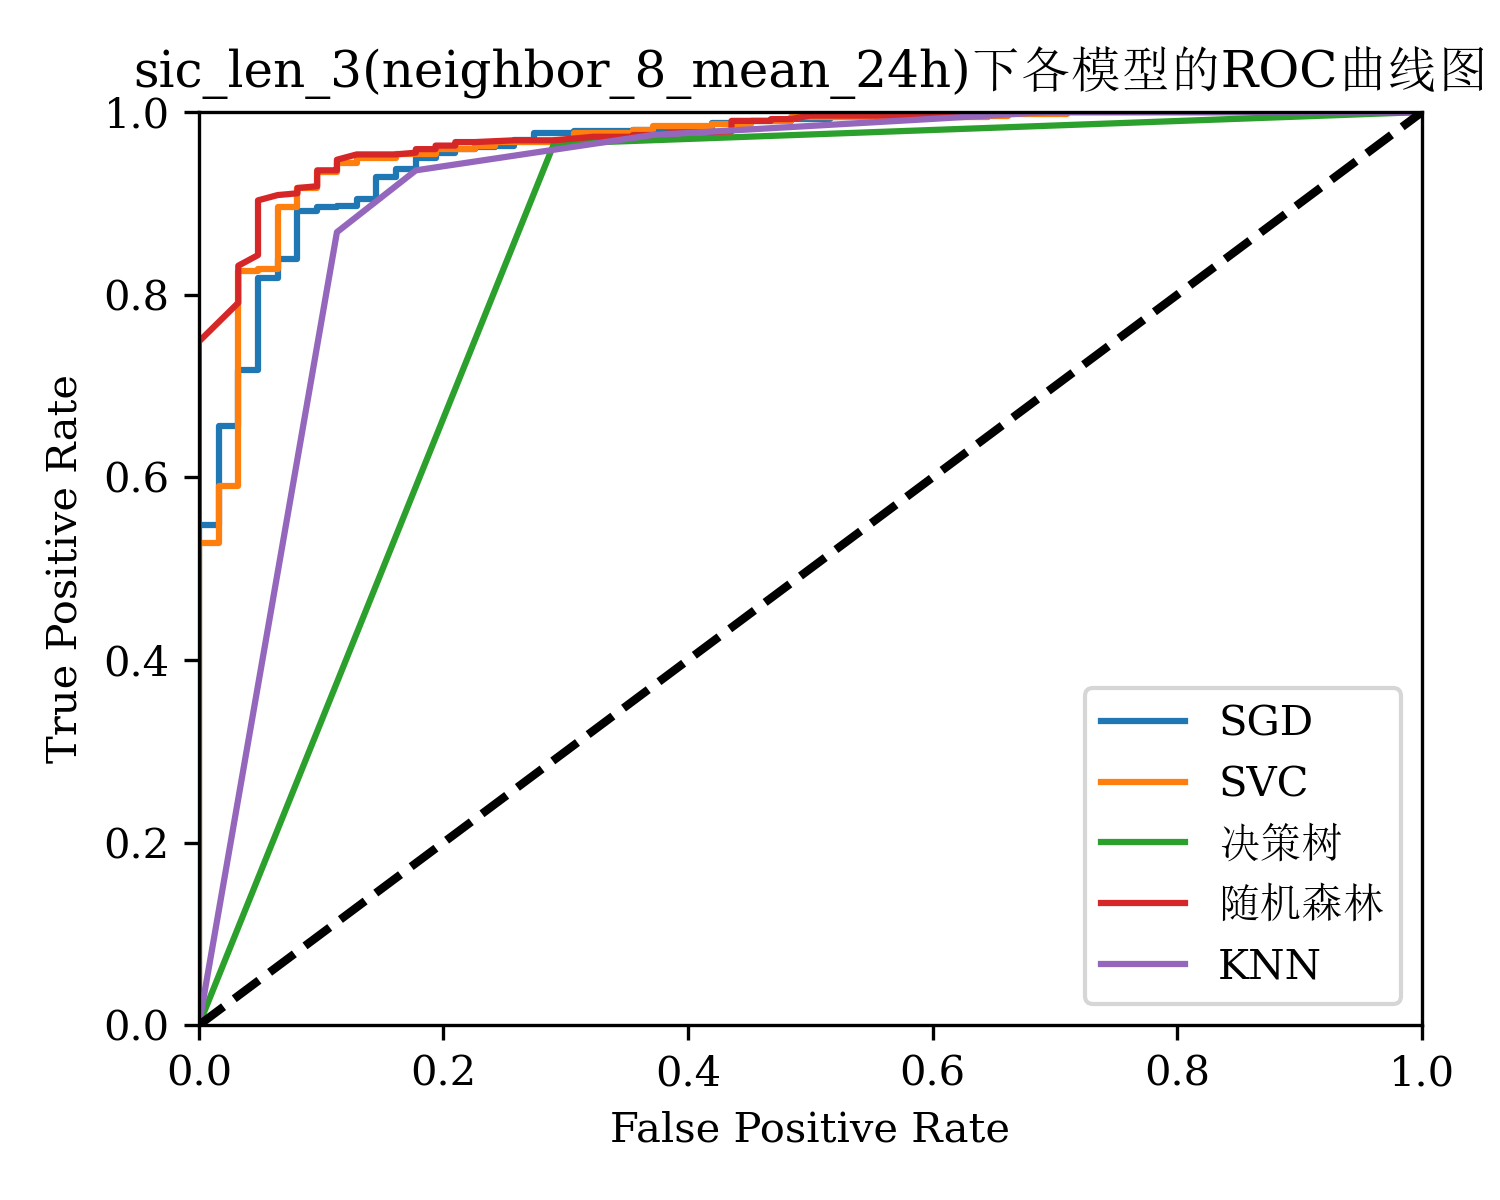
\includegraphics[scale=0.75]{sic_len_3(neighbor_8_mean_24h)_roc_curves.png}
        \caption{不同模型对SIC预测的ROC值}
    \end{subfigure}
    \caption{不同机器学习模型分别对DIC和SIC数据集训练效果比较}
    \label{fig-ML-compare}
\end{figure}
\clearpage
\section{模型可解释性分析}
\subsection{SHAP值基本原理}
\subsection{基于SHAP值的可解释性分析}
借助SHAP分析工具\footnote{\url{https://github.com/slundberg/shap}},我们对数据集分别进行了整体与单个数据的分析。
\subsubsection{整体数据可解释性分析}
我们分别对DIC、SIC的两个最优数据集进行了SHAP值分析,整体分析结果如图\ref{fig-shap-total}所示,这种数据分析图被形象地称作
蜂巢图,其以密度的形式显示数据中的特征如何影响模型的输出,每一行表示一种特征(我们将序列长度编号从0开始,也就是\texttt{pt\_1}
表示第2个信息段中的的凝血原酶时间,如果时间从0开始计算,也就是4到8小时中数据),
其上的每个点表示一个数据的该种特征对其输出的影响大小,
横轴表示该特征的SHAP值,若某个特征在同一个SHAP值处存在多个数据,则会在纵轴上进行堆叠,以显示密度大小。

通过SHAP值的正负可以体现该特征对患病是促进还是抑制,若SHAP为正则说明对患病有正向作用,反之亦然。每个数据点的颜色分布
大小由右侧特征值分布柱给出,通过结合颜色与横轴,可以说明该特征的大小与患病之间的关系。

例如由图\ref{fig-shap-dic}中第2行可以看出,第2个信息段中的D-二聚体\texttt{d\_dim}的与第3个时间段是否患DIC成正相关;
从第5行可以看出,第2个信息段中的血小板计数\texttt{plt}与是否患DIC成负相关。
\begin{figure}[H]
   \hspace{-1.7cm}
   % 如果一行放三个图改成0.3\linewidth即可
   \begin{subfigure}[b]{0.55\textwidth}
       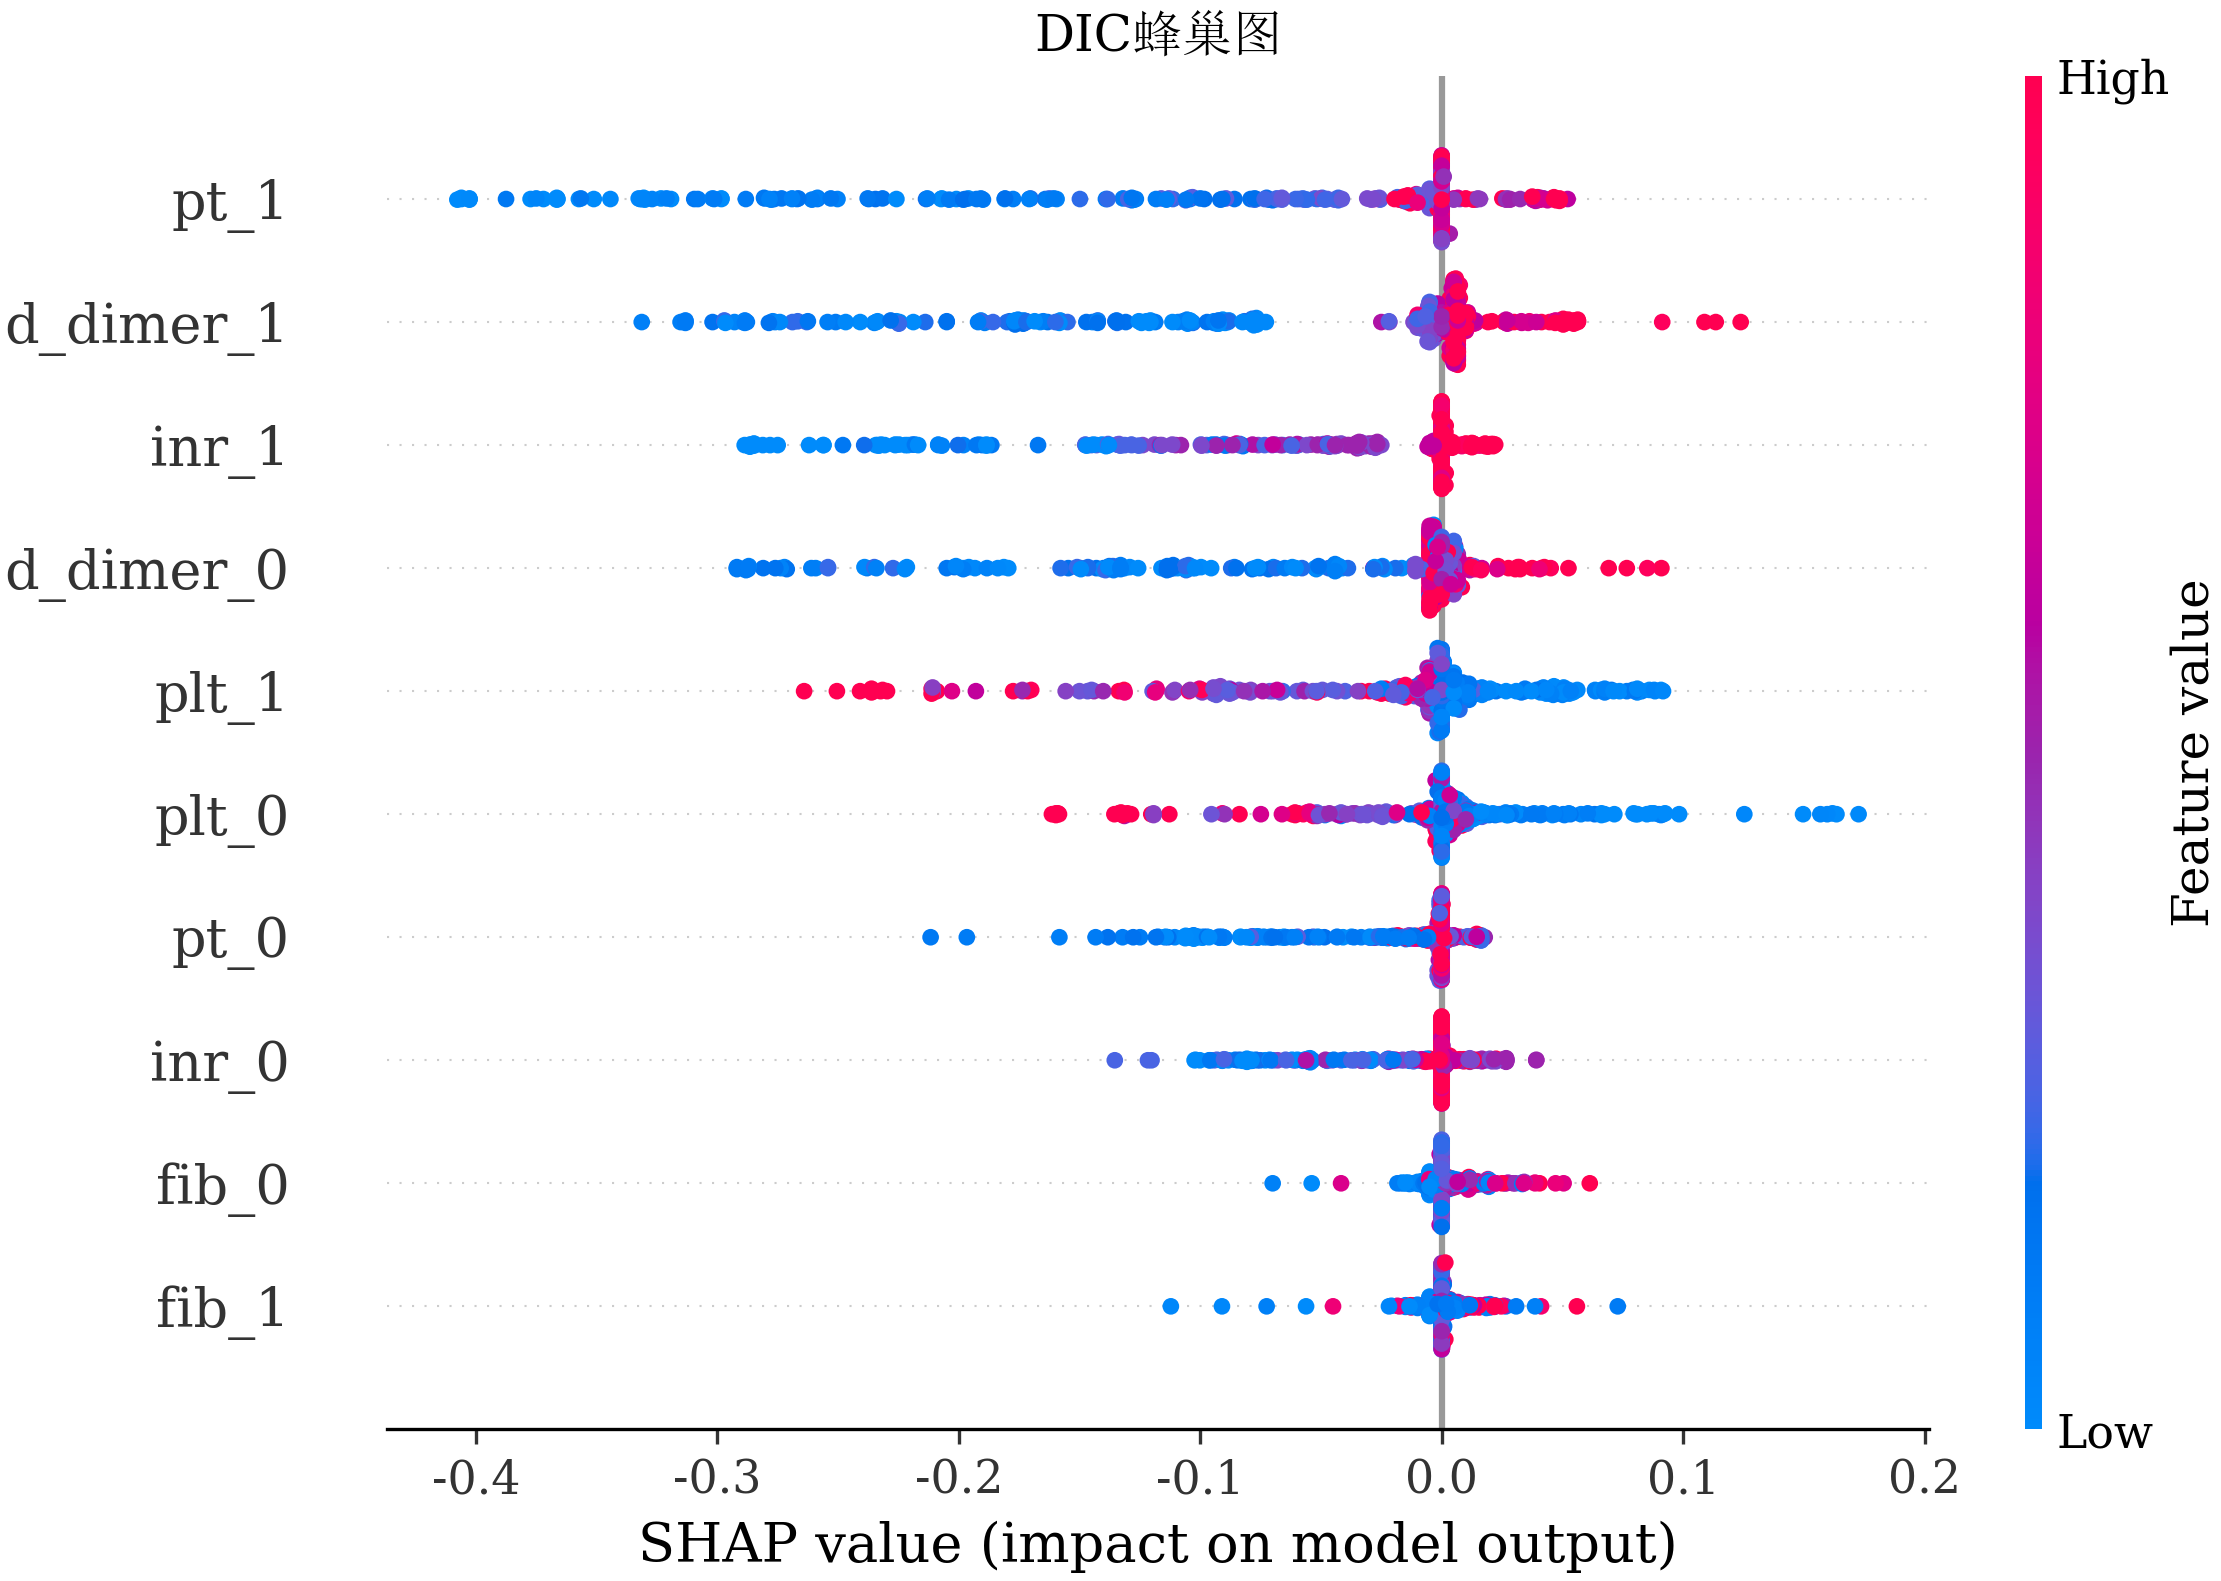
\includegraphics[scale=0.2]{SHAP/shap_dic_beeswarm}
       \caption{DIC特征与SHAP值的关系}
       \label{fig-shap-dic}
   \end{subfigure}
   \begin{subfigure}[b]{0.6\textwidth}
       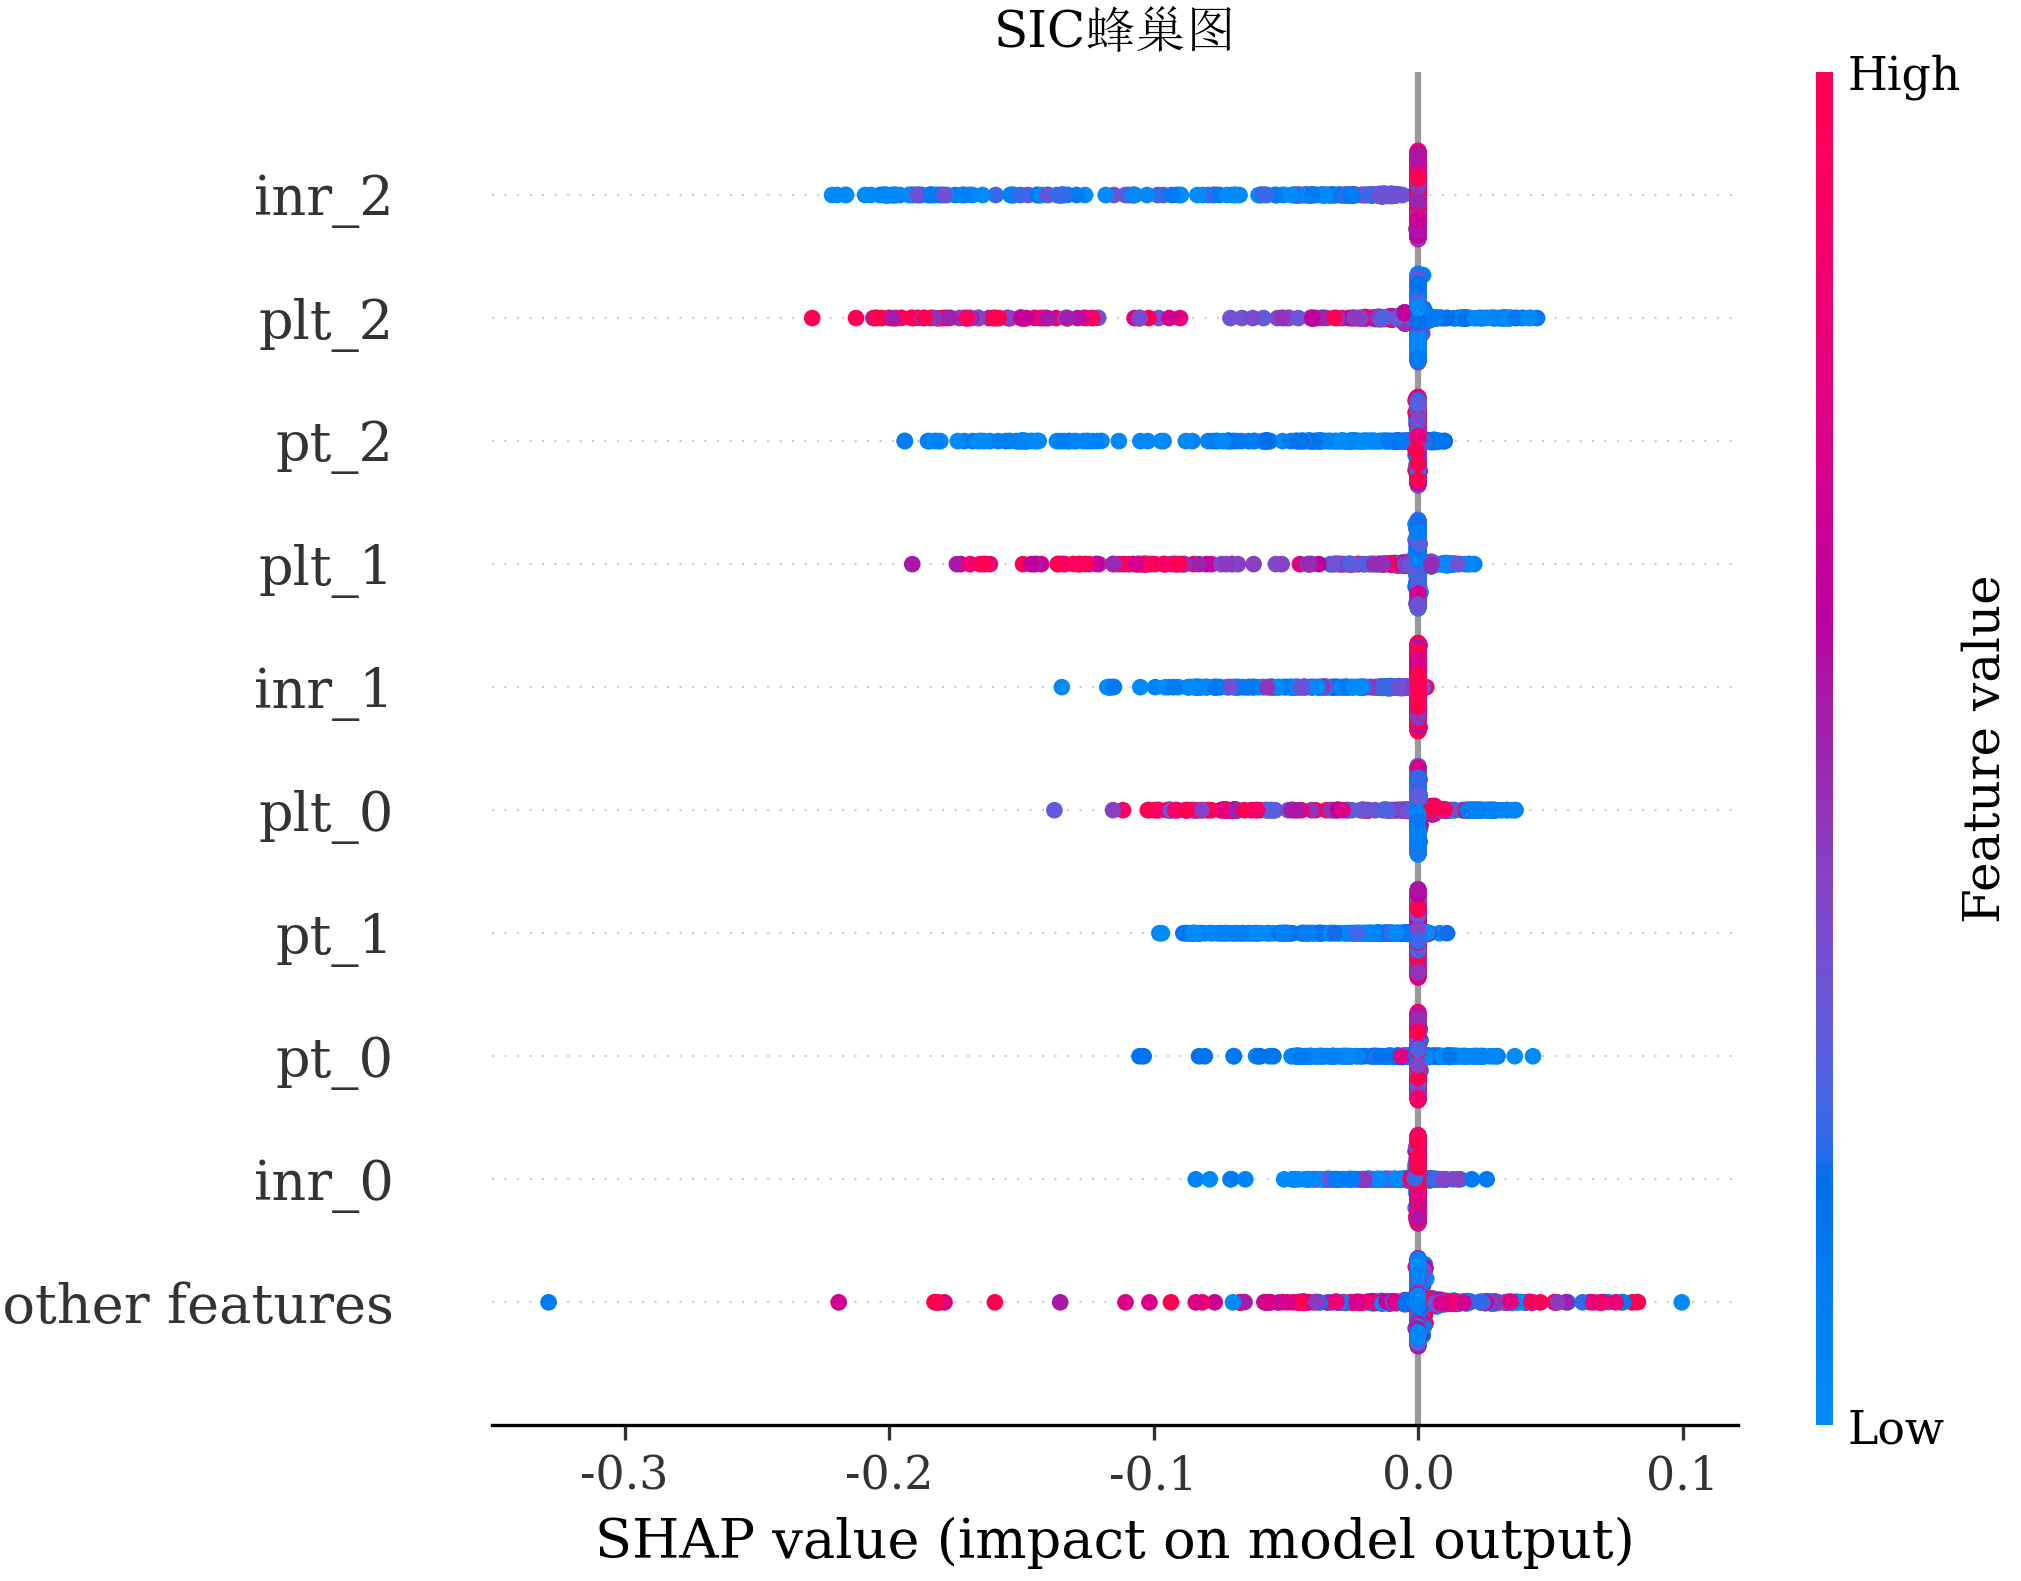
\includegraphics[scale=0.2]{SHAP/shap_sic_beeswarm}
       \caption{SIC特征与SHAP值的关系}
   \end{subfigure}
   \caption{两种指标下的特征与SHAP值之间的关系}
   \label{fig-shap-total}
\end{figure}

更多地,我们通过每个特征的SHAP值均值大小从而用柱状图给出每个特征的重要度排名(附录图\ref{fig-shap-bar}),
将其与随机森林的重要度排名图\ref{fig-ML-compare}相比,可以发现二者排名基本相同,说明SHAP值对模型的解释性是可性信的。

同时我们还给出了两种特征下重要度最高的两个特征的SHAP值与其对应取值的散点图,附录图\ref{fig-shap-scatter}。
\subsubsection{单个数据可解释性分析}
进一步我们可以通过SHAP对单个病人的数据进行分析,从而说明具体哪些特征对患病具有正或负向作用,并说明当前对致病因素的影响最大的特征是什么,
从而为病症的治疗给出相应的建议,图\ref{fig-shap-force}中分别利用强度图\cite{bib-shap-force}给出了两种标签下的影响效应(特征的定义与整体数据分析中给出的定义相同)。

以图\ref{fig-shap-dic-force}为例,该图说明模型对该病人在第3个时间段下患病的预测概率大小为$70\%$,
通过SHAP值给出了每个特征值对预测概率的影响关系,从而我们可以根据SHAP值对病情给出相应的建议。
从该图中可知,第2个时间段下的\texttt{d\_dimer}对患病的正促进作用最大,
而第2个时间段下的\texttt{pt}对患病的抑制作用最大,所以此时的建议应该将尝试降低\texttt{d\_dimer}与\texttt{pt}为主要方向。

以下两个数据更具体影响效果请见附录中瀑布图\ref{fig-shap-waterfall},瀑布图中给出了每个特征的SHAP值对最终预测结果的具体值大小。
\begin{figure}[H]
   % 如果一行放三个图改成0.3\textwidth即可
   \begin{subfigure}[b]{1\textwidth}
       \hspace{-2.6cm}
       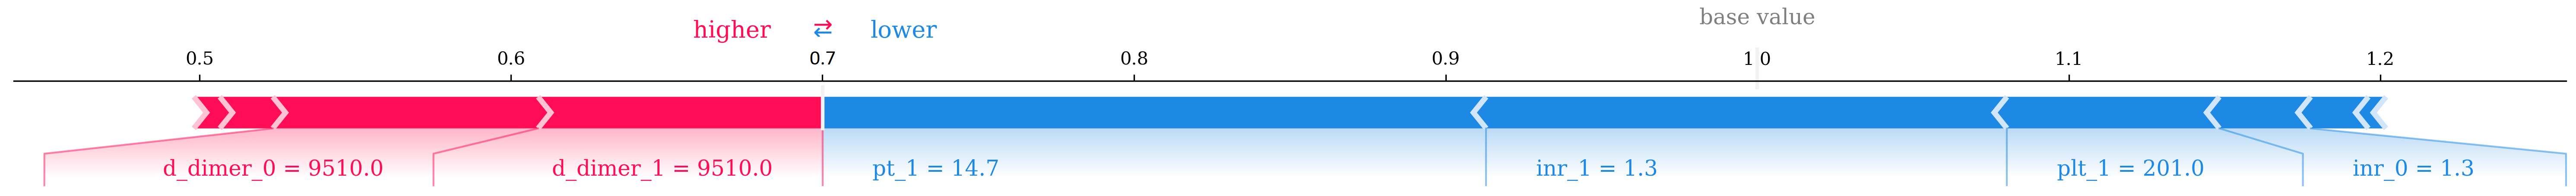
\includegraphics[scale=0.133]{SHAP/单个数据_shap_dic_force}
       \caption{DIC数据中第104号数据强度图分析}
       \label{fig-shap-dic-force}
   \end{subfigure}

   \bigskip
   \begin{subfigure}[b]{1\textwidth}
       \hspace{-2.6cm}
       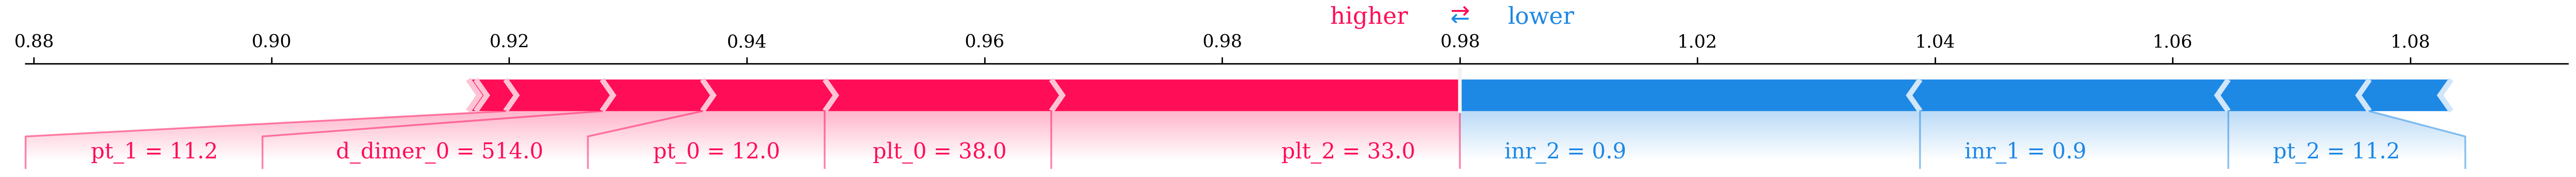
\includegraphics[scale=0.133]{SHAP/单个数据_shap_sic_force}
       \caption{SIC数据中第136号数据强度图分析}
   \end{subfigure}
   \caption{两种指标下的单个数据预测结果与特征之间的关系}
   \label{fig-shap-force}
\end{figure}
\section{结论与展望}
\clearpage
\begin{thebibliography}{99}
    \bibitem{bib-mimic} Johnson, A., Bulgarelli, L., Pollard, T., Horng, S., Celi, L. A., \& Mark, R. (2023). 
    MIMIC-IV (version 2.2)[DB]. PhysioNet. \url{https://doi.org/10.13026/6mm1-ek67}.
    \bibitem{bib-mimic-origin} Johnson, A.E.W., Bulgarelli, L., Shen, L. et al. MIMIC-IV, 
    a freely accessible electronic health record dataset[DB]. Sci Data 10, 1 (2023). 
    \url{https://doi.org/10.1038/s41597-022-01899-x}.
    \bibitem{bib-determine-dic} Toshiaki Iba, Yutaka Umemura, et al. 
    Diagnosis of sepsis-induced disseminated intravascular coagulation and coagulopathy[J]. 
    Acute Medicine \& Surgery(July 2019), Japanese Association for Acute Medicine, Pages 223-232.
    \url{https://doi.org/10.1002/ams2.411}
    \bibitem{bib-shap} Lundberg, Scott M and Lee, Su-In. A Unified Approach to Interpreting Model Predictions[J].
    Advances in Neural Information Processing Systems 30(2017), Curran Associates, Inc.
    \url{https://doi.org/10.48550/arXiv.1705.07874}
    \bibitem{bib-shap-force} Scott M. Lundberg, Bala Nair, et al. 
    Explainable machine-learning predictions for the prevention of hypoxaemia during surgery[J].
    Nature Biomedical Engineering volume 2, pages 749–760 (2018).
    \url{https://doi.org/10.1038/s41551-018-0304-0}
\end{thebibliography}
\clearpage
\appendix
\section{附录}
\subsection{预处理后SIC和DIC数据量}
\renewcommand\arraystretch{1.2} % 设置表格高度为原来的1.2倍
\begin{table}[H] % table标准
    \centering % 表格居中
    \begin{tabular}{p{0.14\textwidth}<{\centering}p{0.11\textwidth}<{\centering}p{0.11\textwidth}
        p{0.25\textwidth}p{0.25\textwidth}} % 设置表格宽度
        \toprule
        \textbf{时间段长度}&\textbf{插补策略}&\textbf{填补策略}&\textbf{SIC标签数量}&\textbf{DIC标签数量}\\
        \midrule
        4h&均值插补&临近填补&827(占比89.89\%)&629(占比68.37\%)\\
        8h&均值插补&临近填补&1885(占比87.55\%)&1345(占比62.47\%)\\
        12h&均值插补&临近填补&1823(占比86.77\%)&1267(占比60.30\%)\\
        \bottomrule
    \end{tabular}
    \caption{预处理后的SIC和DIC数据量}
    \label{table-sic-dic}
\end{table}
\subsection{数据集划分结果}
\renewcommand\arraystretch{1.2} % 设置表格高度为原来的1.2倍
\begin{table}[H] % table标准
    \centering % 表格居中
\begin{tabular}{ccccccc}
        \toprule
\makecell{\textbf{数据集}\\\textbf{时段长度}} & \textbf{序列长度} & \textbf{训练集} & \textbf{测试集} & \textbf{总计} & \textbf{SIC占比} & \textbf{DIC占比} \\
        \midrule
4小时& 1               & 527          & 132          & 659         & 90.44\%        & 70.41\%        \\
4小时& 2               & 318          & 80           & 398         & 92.71\%        & 75.13\%        \\
4小时  & 3               & 208          & 53           & 261         & 93.87\%        & 78.93\%        \\
4小时  & 4               & 132          & 33           & 165         & 95.15\%        & 82.42\%        \\
8小时  & 1               & 1308         & 328          & 1636        & 88.02\%        & 63.75\%        \\
8小时  & 2               & 895          & 224          & 1119        & 88.74\%        & 65.95\%        \\
8小时  & 3               & 579          & 145          & 724         & 89.36\%        & 68.23\%        \\
8小时  & 4               & 330          & 83           & 413         & 90.07\%        & 69.73\%        \\
12小时 & 1               & 1223         & 306          & 1529        & 87.25\%        & 61.81\%        \\
12小时 & 2               & 765          & 192          & 957         & 88.09\%        & 63.64\%        \\
12小时 & 3               & 387          & 97           & 484         & 89.46\%        & 67.98\%        \\
12小时 & 4               & 202          & 51           & 253         & 90.51\%        & 70.75\%       \\
        \bottomrule
\end{tabular}
    \caption{数据集划分结果(均使用临近填充与均值插补)}
    \label{table-divide}
\end{table}
\clearpage
\subsection{模型评估结果}
数据集名称解释:“dic\_len\_1(neighbor\_12\_mean\_24h)”表示预测指标为DIC,基于前1个12小时的信息段,预测后12小时是否患有DIC,
使用临近填充和均值插补。
\renewcommand\arraystretch{1.2} % 设置表格高度为原来的1.2倍
\begin{table}[H] % table标准
    \centering % 表格居中
\begin{tabular}{cccccc}
    \toprule
\textbf{数据集名称}                       & \textbf{SGD} & \textbf{SVC} & \textbf{决策树} & \textbf{随机森林} & \textbf{KNN} \\
    \midrule
dic\_len\_1(neighbor\_12\_mean\_24h) & 0.8497       & 0.8922       & 0.8856       & 0.8954        & 0.8693       \\
dic\_len\_1(neighbor\_4\_mean\_24h)  & 0.8712       & 0.9394       & 0.9318       & 0.9394        & 0.8788       \\
dic\_len\_1(neighbor\_8\_mean\_24h)  & 0.878        & 0.9482       & 0.939        & 0.9482        & 0.9116       \\
dic\_len\_2(neighbor\_12\_mean\_24h) & 0.901        & 0.9115       & 0.901        & 0.9323        & 0.9115       \\
dic\_len\_2(neighbor\_4\_mean\_24h)  & 0.9125       & 0.9625       & 0.9875       & 0.9875        & 0.95         \\
dic\_len\_2(neighbor\_8\_mean\_24h)  & 0.8616       & 0.9286       & 0.9196       & 0.9286        & 0.933        \\
dic\_len\_3(neighbor\_12\_mean\_24h) & 0.8557       & 0.9278       & 0.8763       & 0.9588        & 0.8969       \\
dic\_len\_3(neighbor\_4\_mean\_24h)  & 0.8868       & 0.9434       & 0.9434       & 0.9434        & 0.9245       \\
dic\_len\_3(neighbor\_8\_mean\_24h)  & 0.9034       & 0.9448       & 0.9448       & 0.9793        & 0.9448       \\
dic\_len\_4(neighbor\_12\_mean\_24h) & 0.8431       & 0.9412       & 0.9608       & 0.9804        & 0.9216       \\
dic\_len\_4(neighbor\_4\_mean\_24h)  & 0.9394       & 0.9091       & 0.8182       & 0.9394        & 0.9091       \\
dic\_len\_4(neighbor\_8\_mean\_24h)  & 0.9157       & 0.9398       & 0.9759       & 0.9759        & 0.9277       \\
sic\_len\_1(neighbor\_12\_mean\_24h) & 0.8987       & 0.9248       & 0.9183       & 0.9346        & 0.9346       \\
sic\_len\_1(neighbor\_4\_mean\_24h)  & 0.947        & 0.9621       & 0.9394       & 0.9545        & 0.9394       \\
sic\_len\_1(neighbor\_8\_mean\_24h)  & 0.9329       & 0.9634       & 0.9543       & 0.9665        & 0.9573       \\
sic\_len\_2(neighbor\_12\_mean\_24h) & 0.8854       & 0.9375       & 0.9062       & 0.9427        & 0.9375       \\
sic\_len\_2(neighbor\_4\_mean\_24h)  & 0.9625       & 0.975        & 0.9625       & 0.975         & 0.95         \\
sic\_len\_2(neighbor\_8\_mean\_24h)  & 0.9464       & 0.9643       & 0.9554       & 0.9509        & 0.9241       \\
sic\_len\_3(neighbor\_12\_mean\_24h) & 0.8969       & 0.9485       & 0.9278       & 0.9588        & 0.9485       \\
sic\_len\_3(neighbor\_4\_mean\_24h)  & 0.9811       & 0.9811       & 0.9811       & 0.9811        & 0.9811       \\
sic\_len\_3(neighbor\_8\_mean\_24h)  & 0.9655       & 0.9586       & 0.9448       & 0.9793        & 0.9379       \\
sic\_len\_4(neighbor\_12\_mean\_24h) & 0.9412       & 0.9608       & 0.9804       & 1.0           & 0.9804       \\
sic\_len\_4(neighbor\_4\_mean\_24h)  & 0.9091       & 1.0          & 0.9697       & 1.0           & 0.9697       \\
sic\_len\_4(neighbor\_8\_mean\_24h)  & 0.9277       & 0.9398       & 0.9277       & 0.9639        & 0.9398      \\
    \bottomrule
\end{tabular}
    \caption{五种机器学习模型评估结果比对}
    \label{table-ML-compare}
\end{table}
\subsection{基于SHAP值的可解释性分析}
\begin{figure}[H]
   \hspace{-1.7cm}
   % 如果一行放三个图改成0.3\linewidth即可
   \begin{subfigure}[b]{0.6\textwidth}
       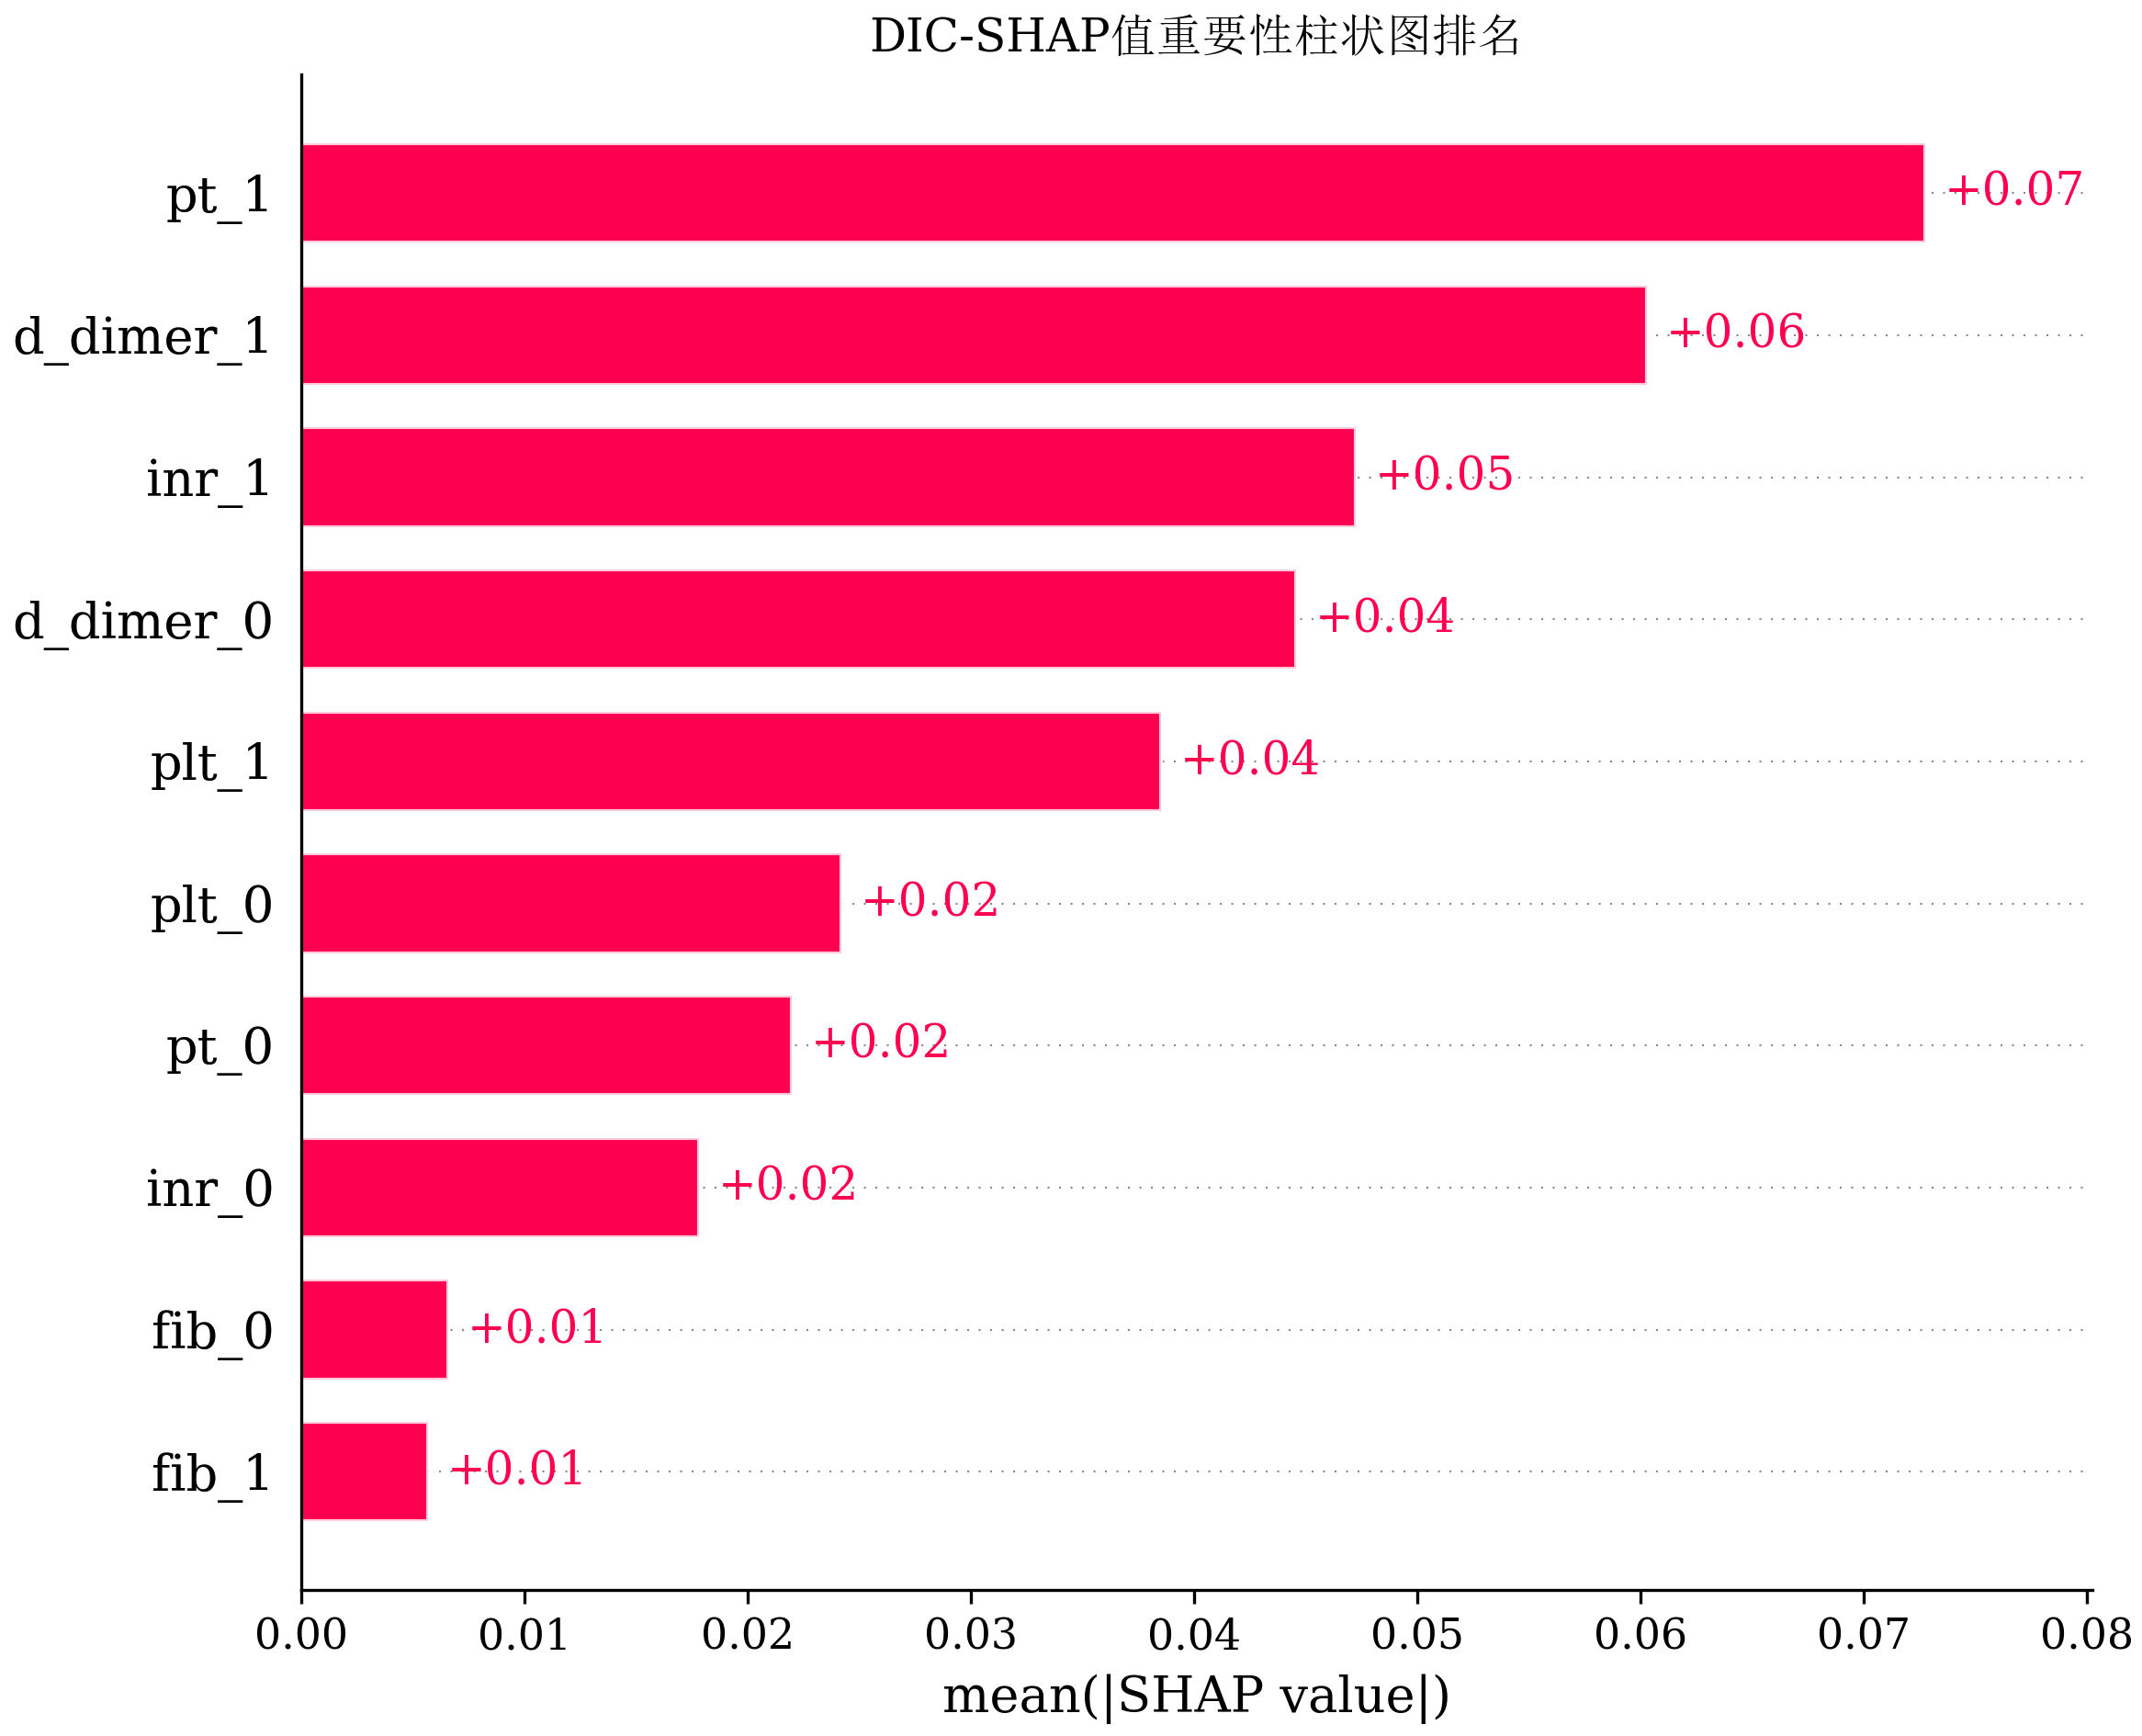
\includegraphics[scale=0.6]{SHAP/shap_dic_bar}
       \caption{DIC特征基于SHAP值的重要度}
   \end{subfigure}
   \begin{subfigure}[b]{0.6\textwidth}
       \includegraphics[scale=0.55]{SHAP/shap_sic_bar}
       \caption{SIC特征基于SHAP值的重要度}
   \end{subfigure}
   \caption{两种指标下的基于SHAP的特征重要度大小}
   \label{fig-shap-bar}
\end{figure}
\begin{figure}[H]
   % 如果一行放三个图改成0.3\linewidth即可
   \begin{subfigure}[b]{1\textwidth}
       \hspace{-1.6cm}
       \includegraphics[scale=0.7]{SHAP/shap_dic_scatter}
       \caption{DIC中的两个关键特征与SHAP值的关系}
   \end{subfigure}

   \bigskip
   \begin{subfigure}[b]{1\textwidth}
       \hspace{-1.6cm}
       \includegraphics[scale=0.7]{SHAP/shap_sic_scatter}
       \caption{SIC中的两个关键特征与SHAP值的关系}
   \end{subfigure}
   \caption{两种指标下的关键特征与SHAP值之间的关系}
   \label{fig-shap-scatter}
\end{figure}
\begin{figure}[H]
   % 如果一行放三个图改成0.3\textwidth即可
   \begin{subfigure}[b]{1\textwidth}
       % \hspace{-1cm}
       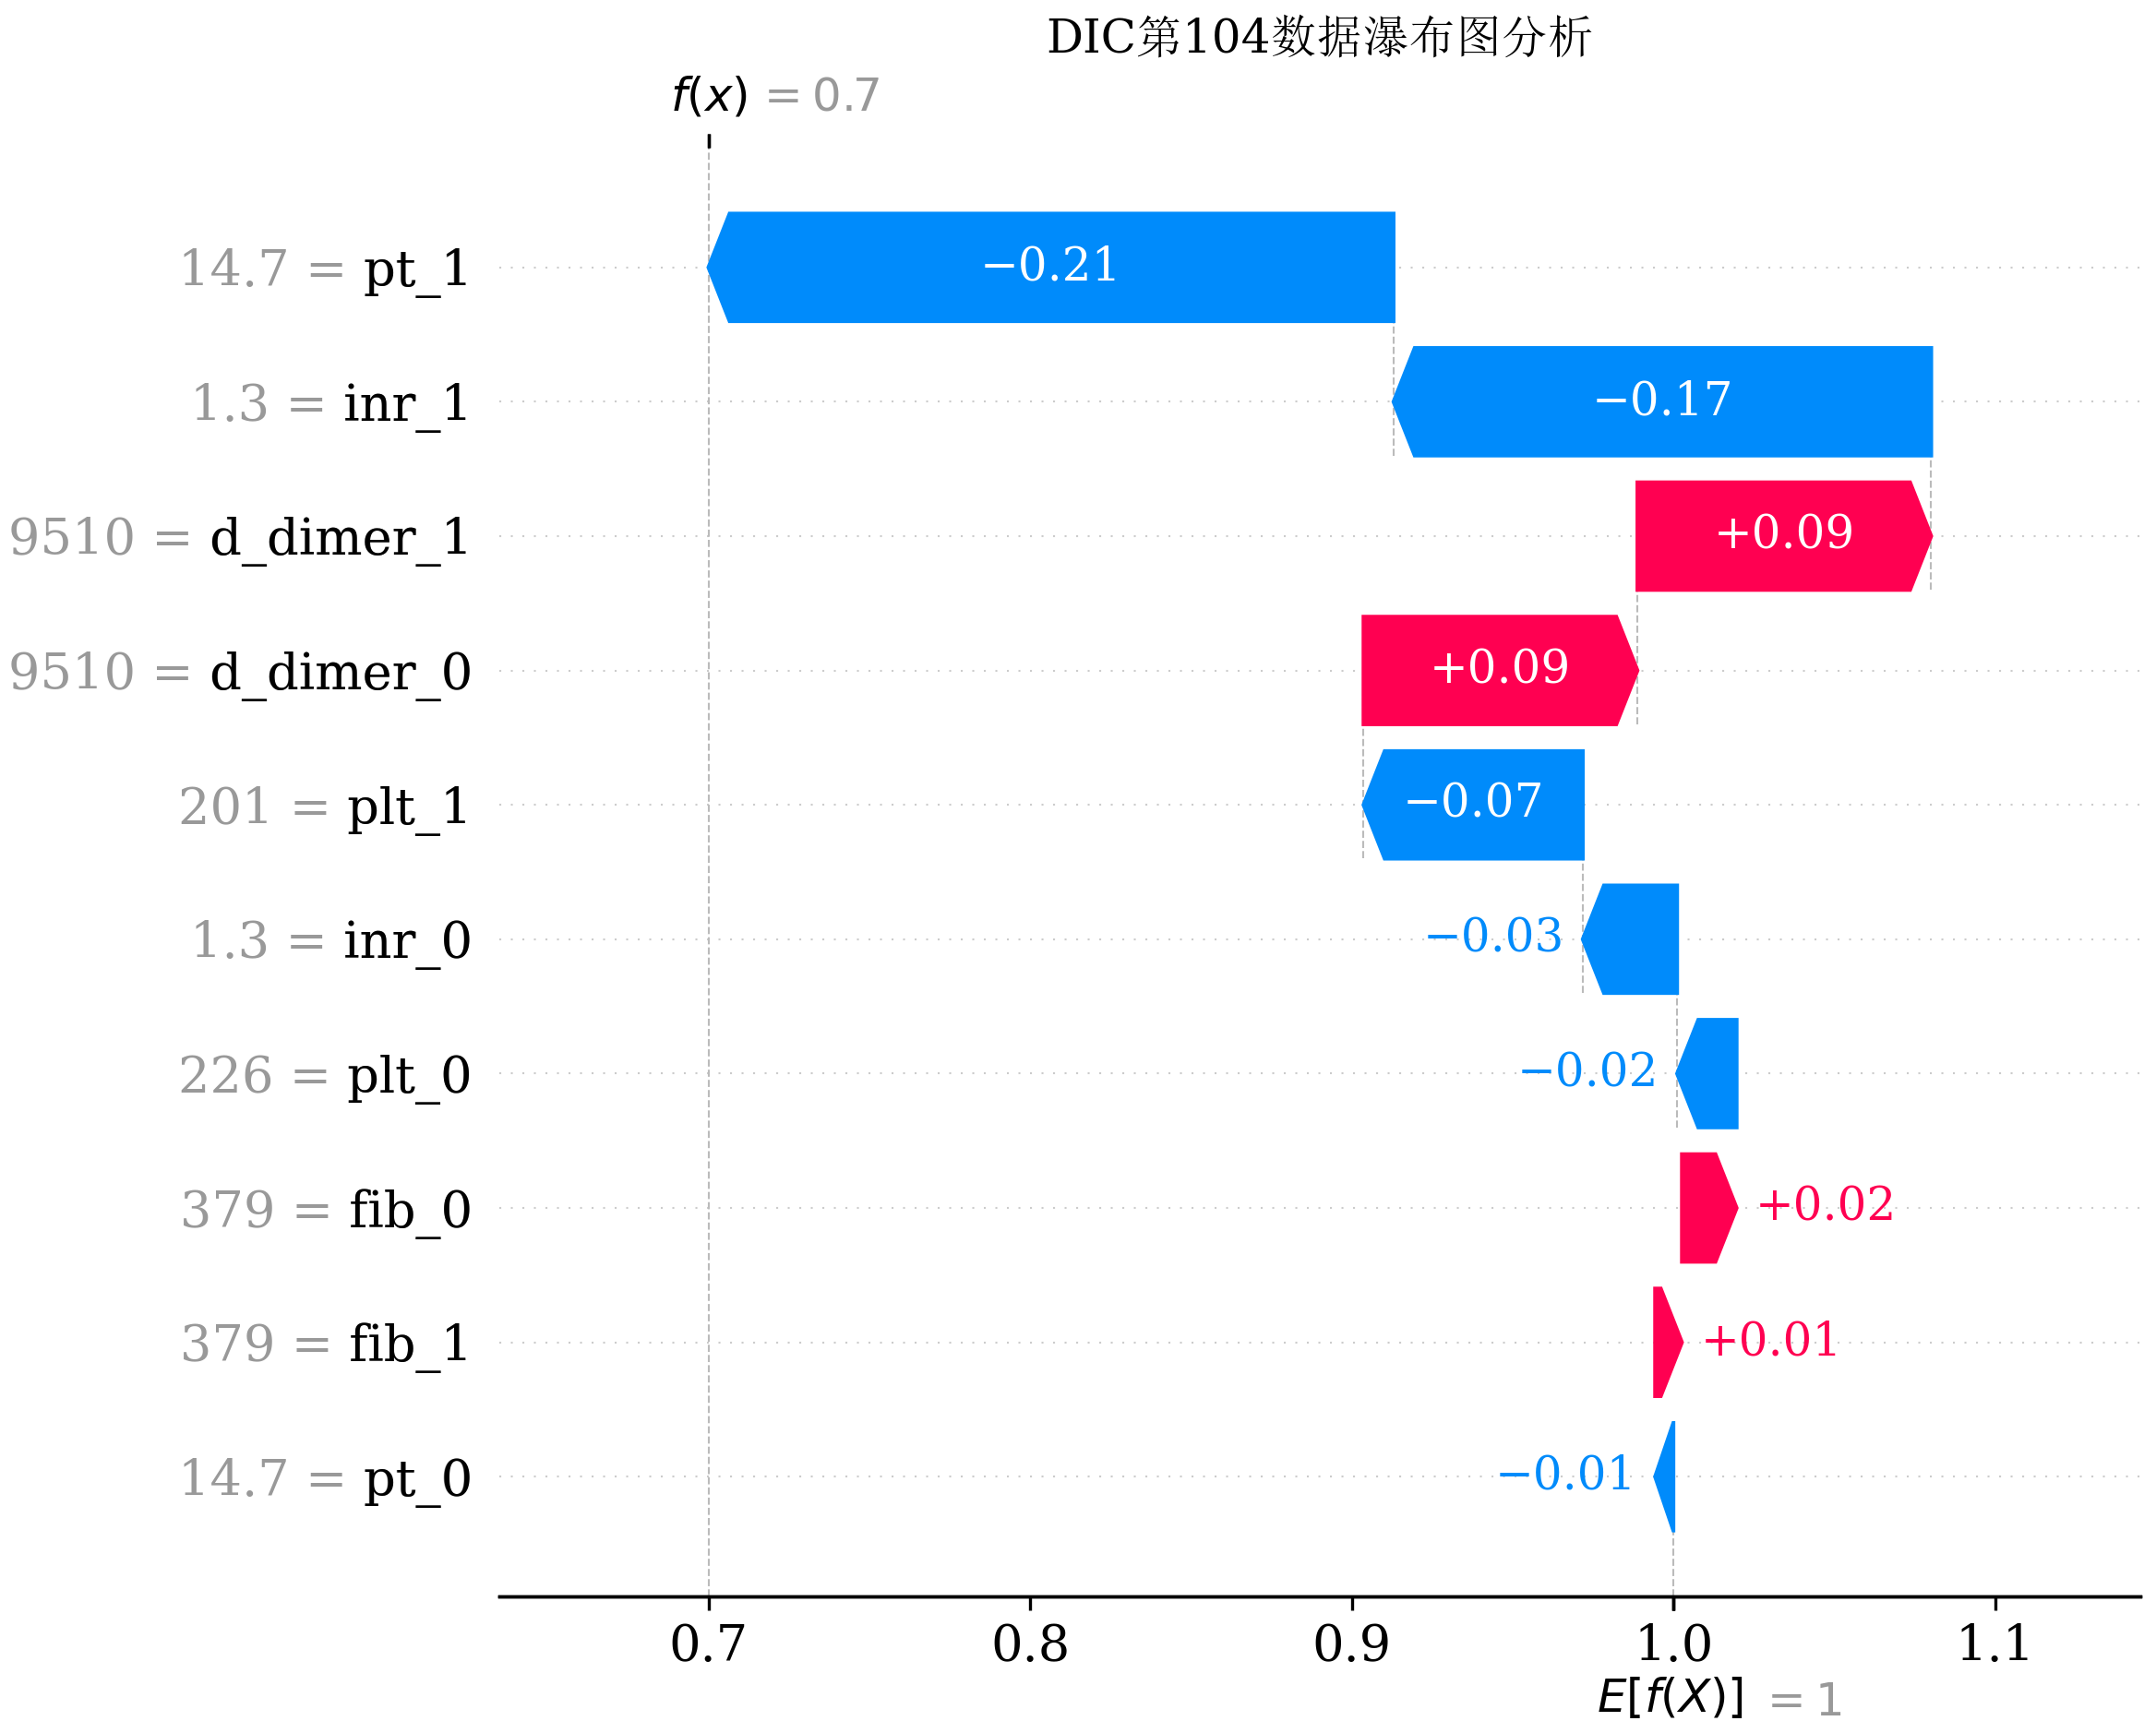
\includegraphics[scale=0.7]{SHAP/单个数据_shap_dic_waterfall}
       \caption{DIC数据中第104号数据瀑布图分析}
   \end{subfigure}

   \bigskip
   \begin{subfigure}[b]{1\textwidth}
       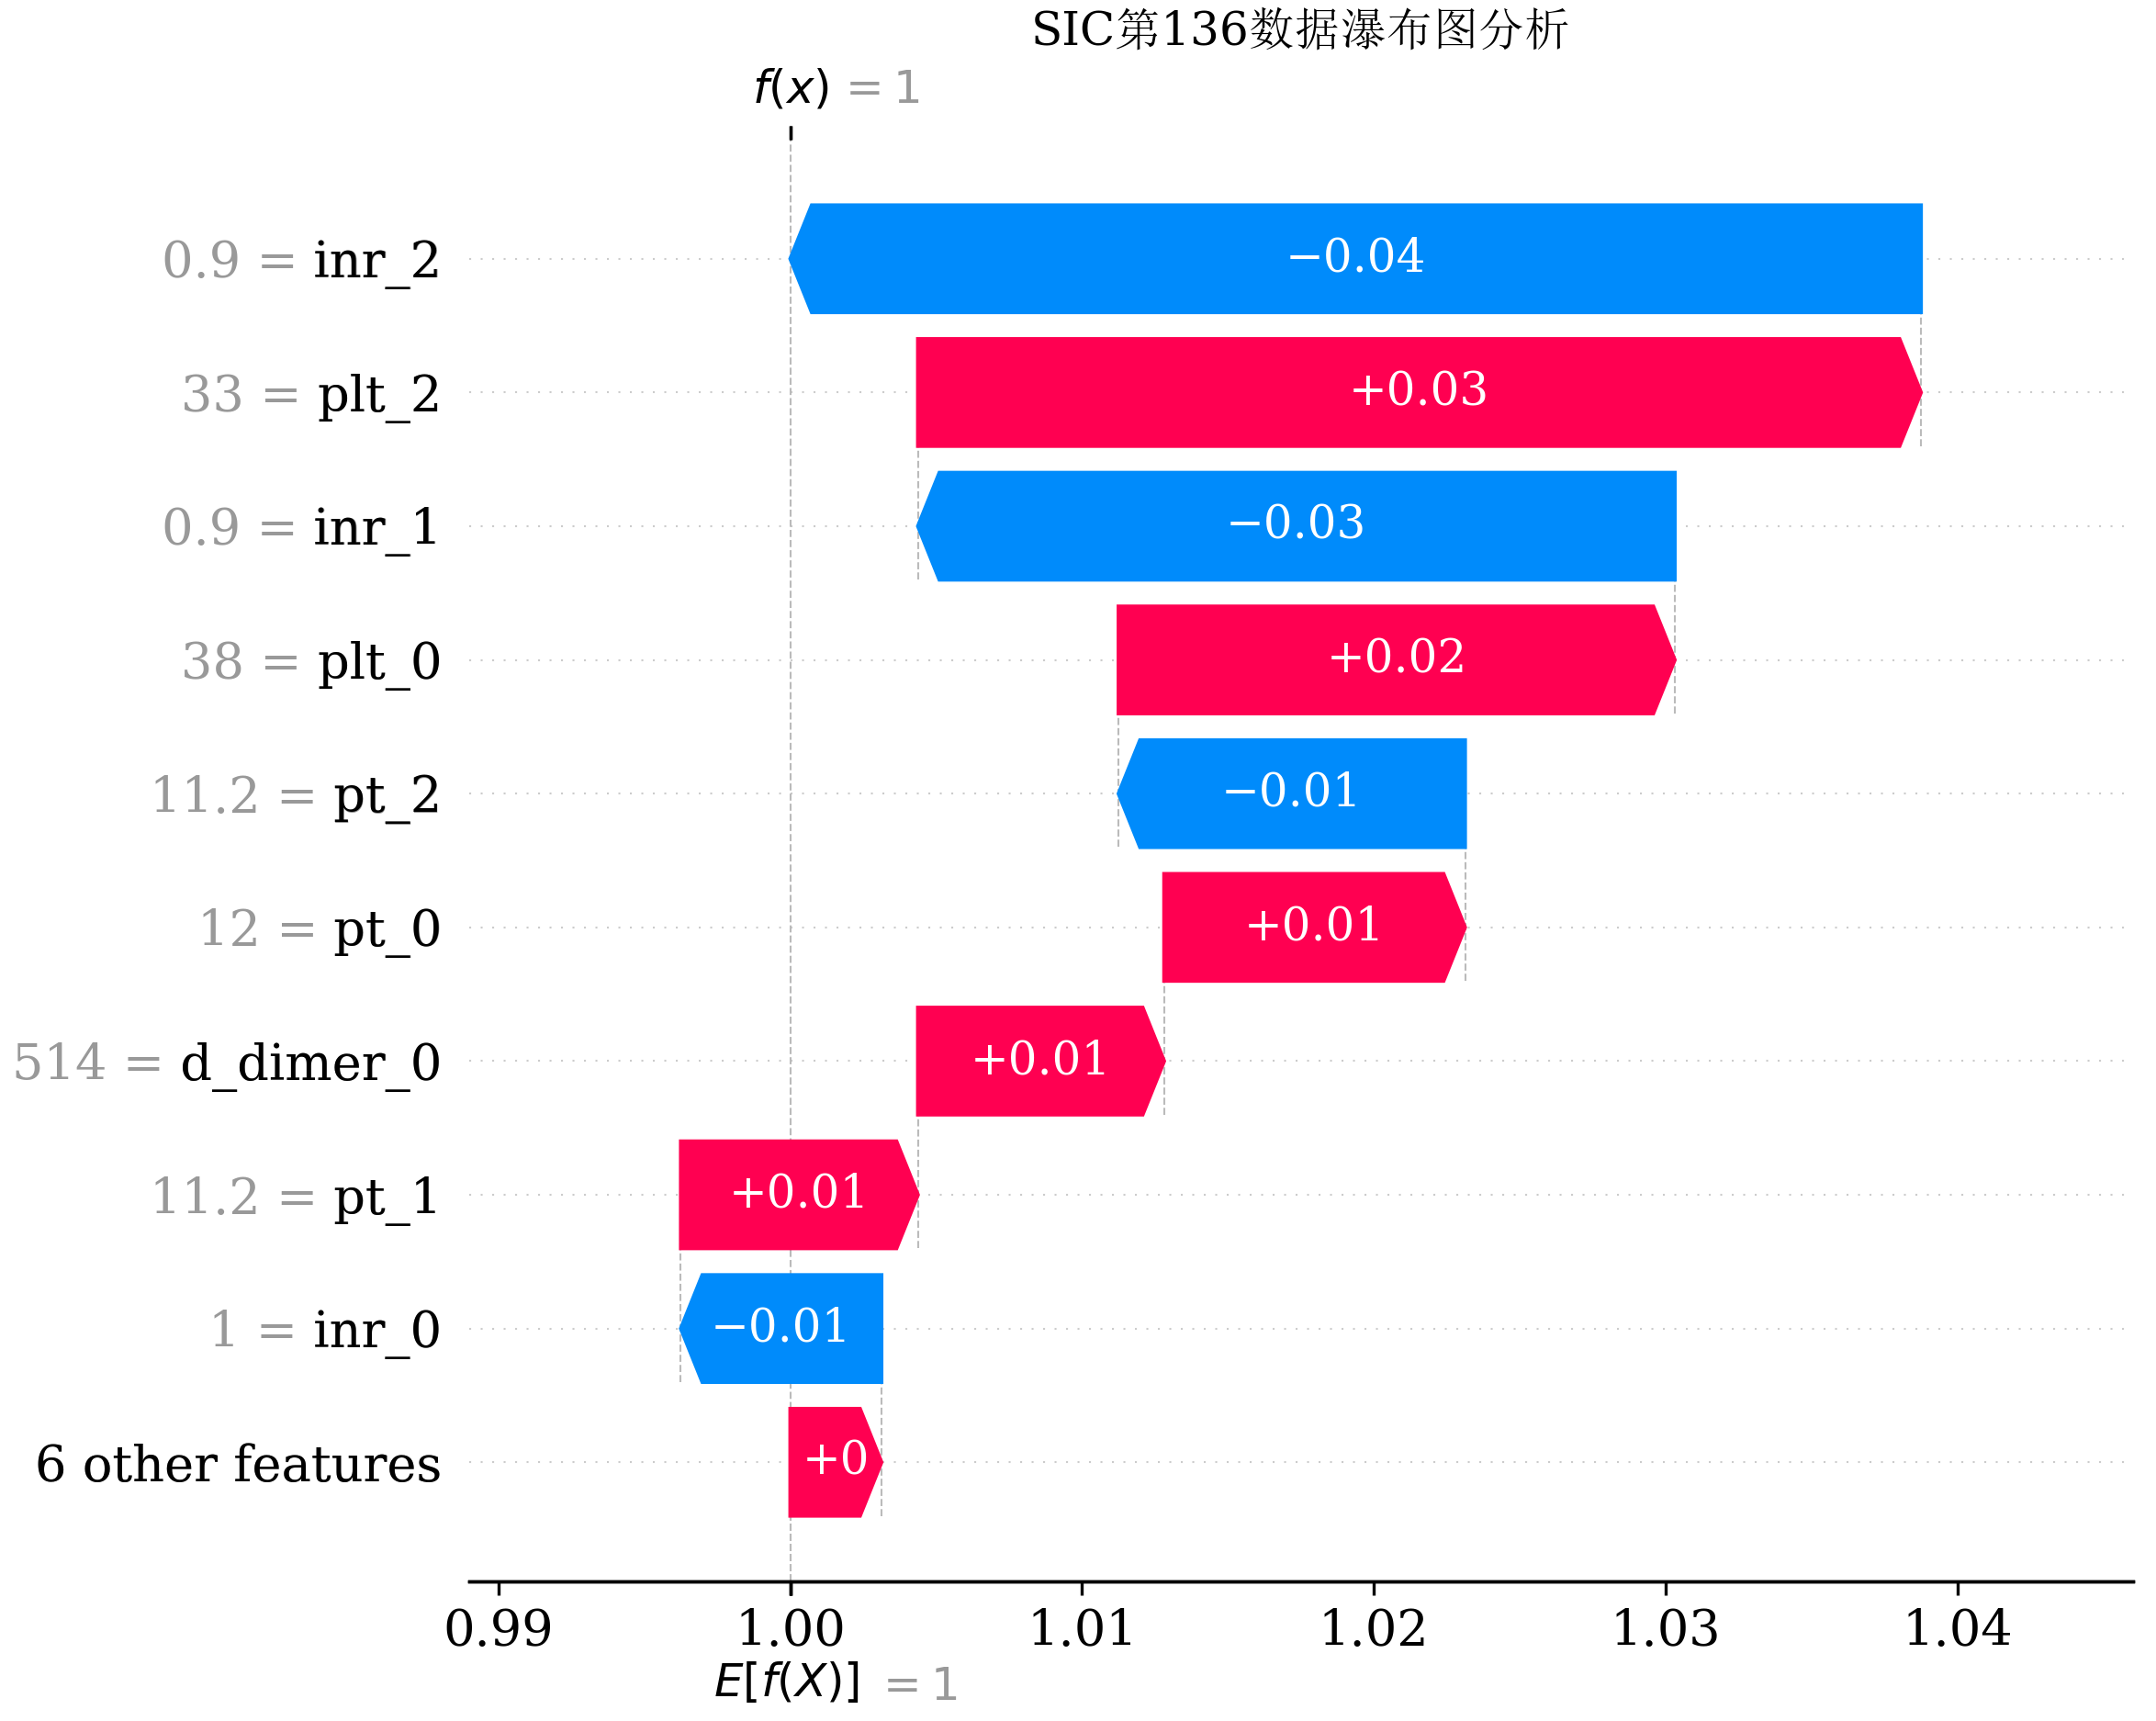
\includegraphics[scale=0.7]{SHAP/单个数据_shap_sic_waterfall}
       \caption{SIC数据中第136号数据瀑布图分析}
   \end{subfigure}
   \caption{两种指标下的单个数据预测结果与特征之间的关系(瀑布图)}
   \label{fig-shap-waterfall}
\end{figure}
\end{document}
